% !TeX spellcheck = en_GB
\chapter{Defects in quantum spin systems}
\label{ch:defects}

In the previous chapter, we have only considered chains with labels from the set of simple objects of a category. However, it is possible to study this setting in a more general way, namely by allowing the labels to come from outside the category. This corresponds to having \emph{defects}\index{defect} in the chain, indicated in red in \cref{fig:defect}.

	\begin{figure}[H]
		\centering
		\begin{tikzpicture}[scale=2]
			\node at (-0.1,0.75) {\textbf{(a)}};
			\draw (0.1,0) -- (4.4,0);
			\draw (0.5,0) -- (0.5,0.5);
			\draw (1,0) -- (1,0.5);
			\draw (1.5,0) -- (1.5,0.5);
			\draw[very thick, LinkColor] (2,0) -- (2,0.5);
			\draw (2.5,0) -- (2.5,0.5);
			\draw (3,0) -- (3,0.5);
			\draw (3.5,0) -- (3.5,0.5);
			\draw (4,0) -- (4,0.5);
%			\node at (0.05,0) {$a$};
			\node at (0.5,0.6) {$a$};
			\node at (1,0.6) {$a$};
			\node at (1.5,0.6) {$a$};
			\node at (2,0.6) {};
			\node at (2.5,0.6) {$a$};
			\node at (3,0.6) {$a$};
%			\node at (4.45,0) {$a$};
			\node at (3.5,0.6) {$a$};
			\node at (4,0.6) {$a$};
			\node at (0.25,-0.15) {$\bullet$};
			\node at (0.75,-0.15) {$\bullet$};
			\node at (1.25,-0.15) {$\bullet$};
			\node at (1.75,-0.15) {$\bullet$};
			\node at (2.25,-0.15) {$\bullet$};
			\node at (2,-0.15) {};
			\node at (2.75,-0.15) {$\bullet$};
			\node at (3.25,-0.15) {$\bullet$};
			\node at (3.75,-0.15) {$\bullet$};
			\node at (4.25,-0.15) {$\bullet$};
		\end{tikzpicture}\\
		\vspace{10pt}
		\begin{tikzpicture}[scale=2]
		\node at (-0.1,0.75) {\textbf{(b)}};
			\draw (0.1,0) -- (4.4,0);
			\draw (0.5,0) -- (0.5,0.5);
			\draw (1,0) -- (1,0.5);
			\draw (1.5,0) -- (1.5,0.5);
			\draw[very thick, LinkColor] (2,0) -- (2,0.5);
			\draw (2.5,0) -- (2.5,0.5);
			\draw (3,0) -- (3,0.5);
			\draw[very thick, LinkColor] (3.5,0) -- (3.5,0.5);
			\draw (4,0) -- (4,0.5);
			%			\node at (0.05,0) {$a$};
			\node at (0.5,0.6) {$a$};
			\node at (1,0.6) {$a$};
			\node at (1.5,0.6) {$a$};
			\node at (2,0.6) {};
			\node at (2.5,0.6) {$a$};
			\node at (3,0.6) {$a$};
			%			\node at (4.45,0) {$a$};
%			\node at (3.5,0.6) {$a$};
			\node at (4,0.6) {$a$};
			\node at (0.25,-0.15) {$\bullet$};
			\node at (0.75,-0.15) {$\bullet$};
			\node at (1.25,-0.15) {$\bullet$};
			\node at (1.75,-0.15) {$\bullet$};
			\node at (2.25,-0.15) {\color{LinkColor} $\bullet$};
			\node at (2,-0.15) {};
			\node at (2.75,-0.15) {\color{LinkColor} $\bullet$};
			\node at (3.25,-0.15) {\color{LinkColor} $\bullet$};
			\node at (3.75,-0.15) {$\bullet$};
			\node at (4.25,-0.15) {$\bullet$};
		\end{tikzpicture}
		\caption{\small \label{fig:defect} \textbf{Defects (red) in a spin chain.} \textbf{(a)} A single defect in a chain constructed from the object $a$, with objects from the category denoted $\bullet$. \textbf{(b)} Having two defects in a chain, the possibilities for objects in between them (red bullets) can be changed.}
	\end{figure}

In general, defects play an important role in the study of \emph{topological phases}\index{topological phase} \cite{Wen1990a,Wen1990b}. Without considering defects, topological phases are already an interesting area in their own right: Due to their insensitivity to environmental noise, they are a promising candidate for topological quantum computation and quantum error-correction \cite{Dennis2002,Kitaev2003,Nayak2008,Terhal2015,Pastawski2015,Brown2016}. The ground space of a topologically ordered system can be used to store quantum data, and by braiding and fusing the emergent quasi-particle excitations it is possible to manipulate the encoded information in a robust manner. However, in many phases (which includes those most suitable for experimental realization) the computational power is severely limited. Here, it has been found that the introduction of defects to the system can enhance the computational power and a lot of work has been done to understand these defects (see, for example, \cite{Fuchs2013,Barkeshli2013,Cong2016,Bridgeman2017,Cong2017,Kesselring2018}).

In this chapter, we study the effects of defects in physical systems via a microscopic approach in order to make sense of a dynamical theory of defects for quantum spin systems. We also discuss how to tackle certain problems in this context with methods from category theory, thereby expanding the chain model we have introduced in the previous chapter. We first discuss defects in topologically ordered systems without using category theory via the two-dimensional toric code example. Then we go into more detail about how to use methods from category theory to make the study of the ground space of the system easier. 

Here, we consider defects in a one-dimensional chain that is built from a fusion category $\C$ (as described in the previous chapter). Defects in this chain are therefore $\C-\C$ bimodules, i.e., we are fusing an element of the category of bimodules to the chain. To realize this, we need to have a description of the corresponding vertices. While in the previous chapter we have only considered vertices within the category, we now need to know how bimodules and objects of the category fuse together. After having constructed the necessary vertices, it is then possible to define a local Hamiltonian from projectors onto simple objects in the same fashion as we did in the previous chapter. We demonstrate how this works with a detailed example, namely a chain constructed from the category $\mathbf{Vec}(\mathbb{Z}/2\mathbb{Z})$, which is the category of vector spaces over the field $\mathbb{Z}/2\mathbb{Z}$ (see \cite{Bridgeman2020}).

This chapter does not directly contribute to answering the central question of this thesis, namely whether there is a CFT that corresponds to the Haagerup subfactor. However, adding defects to an anyon chain is a natural generalisation of the anyon chains studied in the previous chapter and an interesting topic by itself because of its connection to topological phases, hence we study these systems here. Furthermore, the construction of the vertices of the $\mathbf{Vec}(\mathbb{Z}/2\mathbb{Z})$ chain with defects yields insight into how computations are done within the so-called annular category. This category is interesting with regard to UMTCs since there is a connection between the simple objects of the Drinfeld centre of a category and representations of the annular category, which we elaborate on later in this chapter. 


\section{Gauging defects in lattice systems}

Adding defects to a physical system in general changes its dynamical behaviour. Consider a system where each particle is described by the Hilbert space $\mathbb{C}^d$. An example for a two-dimensional system that is often considered is a two-dimensional regular lattice on a torus as depicted in \cref{fig:torus}, which for instance appears in Kitaev's toric code \cite{Kitaev2003}\index{toric code}. In the following, we illustrate the concept of defects by missing spin defects in a lattice on a torus. The Hilbert space of a general lattice system with an unknown number of such particles is given by the \emph{distinguishable Fock space}\index{Fock space}\footnote{At first sight, it seems counter-intuitive that we do not know how many particles we have but still can individually identify and address the particles. A physical example of such a system is a one-dimensional optical lattice in which at each site we either have zero atoms or one two-level atom. We furthermore assume that the atoms are lined up in a contiguous line with no gaps (which can be achieved by imposing some kind of potential gradient). In the resulting lattice we can identify and address the individual atoms via their lattice position, although we do not know the total number of particles.}

\begin{figure}[t]
	\centering
	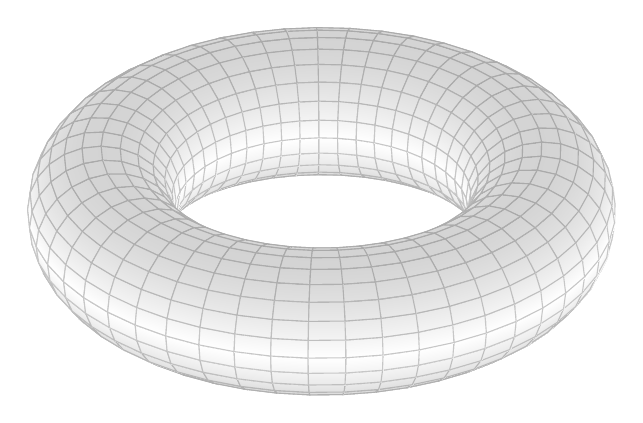
\begin{tikzpicture}
	\begin{axis}[
	axis equal image,
	hide axis,
	z buffer = sort,
	view = {122}{30},
	colormap={mycolormap}{color=(LightGray) color=(white) color=(LightGray)},
	scale = 1.5
	]
	\addplot3[
	surf,
	shader = faceted interp,
	samples = 25,
	samples y= 50,
	domain = 0:2*pi,
	domain y = 0:2*pi,
	colormap name = mycolormap,
	thin
	] (
	{(3+sin(deg(\x)))*cos(deg(\y))},
	{(3+sin(deg(\x)))*sin(deg(\y))},
	{cos(deg(\x))}
	);
	\end{axis}
	\end{tikzpicture}
	\caption{\small \label{fig:torus}\textbf{Lattice on a torus.} This is an example for a two-dimensional lattice with periodic boundary conditions.}
\end{figure}

\begin{equation}
\mathfrak{F}\big(\mathbb{C}^d\big)\cong\bigoplus_{N=0}^\infty\Hi_N\cong\bigoplus_{N=0}^\infty\big(\underbrace{\mathbb{C}^d\otimes\mathbb{C}^d\otimes\dots\otimes\mathbb{C}^d}_{N\ \mathrm{factors}}\big)
\end{equation}
with the convention that the space that describes zero particles (i.e., the vacuum), is described by the Hilbert space  $(\mathbb{C}^d)^{\otimes 0}\cong\mathbb{C}$. We can incorporate defects to this system in the following way: For instance, if a system (with a single site) is comprised of either zero quantum spins or one distinguishable quantum spin, the Hilbert space is given by
\begin{equation}
\label{eq:Fockone}
\mathfrak{F}_{\le 1}\big(\mathbb{C}^d\big)\cong\mathbb{C}\oplus\mathbb{C}^d.
\end{equation}
Here, the subscript indicates that we have at most one quantum spin present in the system. 

Suppose now that we have a system with $n$ sites, where on each site there either is a quantum spin present or not. The absence of a spin corresponds to a defect\footnote{Note that choosing the defect to be an absent spin is only one possible choice. The construction works for arbitrary defects and also situations where different kinds of defects are present in the same system, although the description might become more complicated.} in the system. We can write the overall Hilbert space of the system as a tensor products of single-site Hilbert spaces \cref{eq:Fockone}:
\begin{equation}
\label{eq:Fnone}
\mathfrak{F}_{\le n}\big(\mathbb{C}^d\big)\equiv\bigotimes_{j=0}^n\mathfrak{F}_{\le 1}\big(\mathbb{C}^d\big)\cong\big(\mathbb{C}\oplus\mathbb{C}^d\big)^{\otimes n},
\end{equation}
which can be rewritten by expanding out the tensor factors as
\begin{equation}
\label{eq:Fntwo}
\mathfrak{F}_{\le n}\big(\mathbb{C}^d\big)\cong\bigoplus_{j=0}^n\mathbb{C}^{\binom{n}{j}}\otimes\Hi_j,
\end{equation}
where $\Hi_j=(\mathbb{C}^d)^{\otimes j}$ is the Hilbert space of $j$ distinguishable spins. We can understand this representation as follows: The space $\mathbb{C}^{\binom{n}{j}}$ can be interpreted as the configuration space of $j$ identical scalar particles arranged on a system of $n$ sites, i.e., it takes care of identifying which locations are occupied with spins, while $\Hi_j$ represents the actual distinguishable spins at those positions. At first sight, it is not clear that \cref{eq:Fnone} and \cref{eq:Fntwo} yield the same representation. A quick way to convince yourself that they are actually equal is by checking their respective dimensions. In the first case \cref{eq:Fnone}, we have
\begin{equation}
\dim\Big(\mathfrak{F}_{\le n}\big(\mathbb{C}^d\big)\Big)=\dim\Big(\big(\mathbb{C}\oplus\mathbb{C}^d\big)^{\otimes n}\Big)=(d+1)^n.
\end{equation}
In the second case \cref{eq:Fntwo} we get
\begin{equation}
\dim\Big(\mathfrak{F}_{\le n}\big(\mathbb{C}^d\big)\Big)=\sum_{j=0}^n\binom{n}{j}d^j=(d+1)^n,
\end{equation}
where the last equality is a consequence of the binomial theorem. An example for the different defect configurations that can appear in a higher-dimensional lattice system are given in \cref{fig:defect}. As we will see in the example of the toric code, different configurations of the same number of defects can result in different dimensions of the ground space of the system.

\begin{figure}[t]
	\centering
	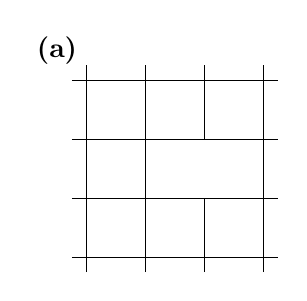
\begin{tikzpicture}[scale=0.75]
	\node at (-0.5,3.5) {\textbf{(a)}};
	\draw (-0.25,0) -- (3.25,0);
	\draw (-0.25,1) -- (3.25,1);
	\draw (-0.25,2) -- (3.25,2);
	\draw (-0.25,3) -- (3.25,3);
	\draw (0,-0.25) -- (0,3.25);
	\draw (1,-0.25) -- (1,3.25);
	\draw (2,-0.25) -- (2,1);
	\draw (2,2)-- (2,3.25);
	\draw (3,-0.25) -- (3,3.25);
	\end{tikzpicture}\hspace{10pt}
	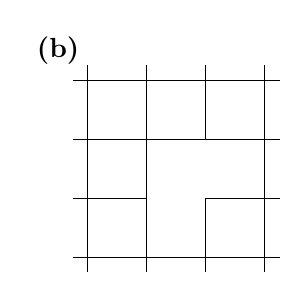
\begin{tikzpicture}[scale=0.75]
	\node at (-0.5,3.5) {\textbf{(b)}};
	\draw (-0.25,0) -- (3.25,0);
	\draw (-0.25,1) -- (1,1);
	\draw (2,1) -- (3.25,1);
	\draw (-0.25,2) -- (3.25,2);
	\draw (-0.25,3) -- (3.25,3);
	\draw (0,-0.25) -- (0,3.25);
	\draw (1,-0.25) -- (1,3.25);
	\draw (2,-0.25) -- (2,1);
	\draw (2,2)-- (2,3.25);
	\draw (3,-0.25) -- (3,3.25);
	\end{tikzpicture}\hspace{10pt}
	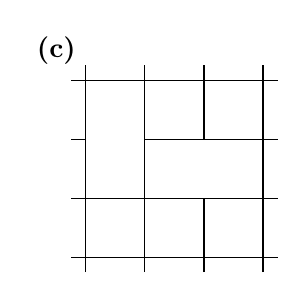
\begin{tikzpicture}[scale=0.75]
	\node at (-0.5,3.5) {\textbf{(c)}};
	\draw (-0.25,0) -- (3.25,0);
	\draw (-0.25,1) -- (3.25,1);
	\draw (-0.25,2) -- (0,2);
	\draw (1,2) -- (3.25,2);
	\draw (-0.25,3) -- (3.25,3);
	\draw (0,-0.25) -- (0,3.25);
	\draw (1,-0.25) -- (1,3.25);
	\draw (2,-0.25) -- (2,1);
	\draw (2,2)-- (2,3.25);
	\draw (3,-0.25) -- (3,3.25);
	\end{tikzpicture}
	\caption{\small \label{fig:2Ddefects} \textbf{Defect configurations in a two-dimensional lattice.} \textbf{(a)} A single defect. \textbf{(b)} Two adjacent defects. \textbf{(c)} Two distant defects: This configuration gives rise to a different ground space than two adjacent defects.}
\end{figure}

The Hilbert space $\mathfrak{F}_{\le n}\big(\mathbb{C}^d\big)$ provides the kinematical data to describe a system of at most $n$ defects on a lattice with $n$ sites. We now want to incorporate \emph{dynamics} to this system. In quantum mechanics, this is usually done via a Hamiltonian $H$ such that the time evolution of the system is given by
\begin{equation}
\label{eq:timeev}
U_t=e^{-itH}.
\end{equation}
Hence, introducing dynamics on the lattice system described above requires finding a Hermitian matrix that acts on $\mathfrak{F}_{\le n}\big(\mathbb{C}^d\big)$. Although this sounds simple in the abstract, there is a way to introduce dynamical information more indirectly, which is particularly helpful when considering topologically ordered systems such as the toric code.

Instead of specifying the time evolution operator in \cref{eq:timeev} we introduce dynamical information indirectly by describing the ground space $\mathcal{V}\subset\mathcal{H}$ of a specific Hamiltonian $H$. We show how this works with the example of Kitaev's toric code. Here, we have a two-dimensional lattice on a torus as depicted in \cref{fig:torus}. For simplicity we usually do not draw the torus but a simpler, two-dimensional version of the lattice with periodic boundary conditions that is equivalent to the lattice on the torus, for example a $n\times n$ lattice is depicted

\begin{figure}[H]
	\centering	
	\begin{tikzpicture}[scale=0.65]
	\foreach \a in {0,1,...,7}{
		\draw (\a,0) -- (\a,7);	
		\draw (0,\a) -- (7,\a);			
	}
	\draw[LinkColor, very thick] (0,0) -- (7,0);
	\draw[LinkColor, very thick] (0,7) -- (7,7);
	\draw[LinkColor2, very thick] (0,0) -- (0,7);
	\draw[LinkColor2, very thick] (7,0) -- (7,7);
	%			\node at (3.5,0) {//};
	%			\node at (3.5,7) {//};
	%			\node[rotate=-90] at (0,3.5) {$\backslash\backslash$};
	%			\node[rotate=-90] at (7,3.5) {$\backslash\backslash$};
	\node at (0,-0.5) {\small $(1,1)$};
	\node at (6,-0.5) {\small $(n,1)$};
	\node at (-1,6) {\small $(1,n)$};
	%			\node at (6.25,7.4) {\small $(N,M)$};
	\node at (0,0) {$\bullet$};
	\node at (0,6) {$\bullet$};
	\node at (6,0) {$\bullet$};
	%			\node at (6,6) {$\bullet$};
	\end{tikzpicture}
\end{figure}

Here, we identify the upper and the lower line (red) and the left and the right line (blue), respectively, to get the same boundary conditions that we have on a torus. The particles we consider are spins that can either be in the up state or in the down state, hence the single-site Hilbert space is $\mathbb{C}^2$. The overall Hilbert space of the system is then
\begin{equation}
\mathcal{H}_\mathbb{T} =\bigoplus_{j=1}^{n^2}\mathbb{C}^2.
\end{equation}
The Hamiltonian in this case consists of two kinds of terms: Vertex operators that apply a Pauli-$Z$ operator to each edge adjacent to a vertex $\mathbf{v}$ and plaquette operators that apply a Pauli-$X$ operator to each edge of a plaquette $\mathbf{p}$:
\begin{equation}
\label{eq:TCham}
H_\mathbb{T}=-\sum_\mathbf{v}
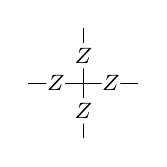
\begin{tikzpicture}[scale=1.4,baseline={([yshift=-3pt]current bounding box.center)}]
\draw (0,0.5) -- (1,0.5);
\draw (0.5,-0) -- (0.5,1);
\draw[fill=white,draw=white] (0.25,0.5) circle (0.08cm);
\draw[fill=white,draw=white] (0.5,0.25) circle (0.11cm);
\draw[fill=white,draw=white] (0.75,0.5) circle (0.08cm);
\draw[fill=white,draw=white] (0.5,0.75) circle (0.11cm);
\node at (0.25,0.5) {\footnotesize $Z$};
\node at (0.5,0.25) {\footnotesize $Z$};
\node at (0.75,0.5) {\footnotesize $Z$};
\node at (0.5,0.75) {\footnotesize $Z$};
\end{tikzpicture}
-\sum_\mathbf{p}
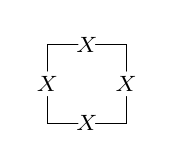
\begin{tikzpicture}[baseline={([yshift=-3pt]current bounding box.center)}]
\draw (0,0) -- (0,1) -- (1,1) -- (1,0) -- cycle;
\draw[fill=white,draw=white] (0.5,0) circle (0.1cm);
\draw[fill=white,draw=white] (0,0.5) circle (0.15cm);
\draw[fill=white,draw=white] (0.5,1) circle (0.1cm);
\draw[fill=white,draw=white] (1,0.5) circle (0.15cm);
\node at (0.5,0) {\footnotesize $X$};
\node at (1,0.5) {\footnotesize $X$};
\node at (0.5,1) {\footnotesize $X$};
\node at (0,0.5) {\footnotesize $X$};
\end{tikzpicture}.
\end{equation}
If we consider a regular $n\times n$ lattice on the torus without any defects, the ground eigenspace $\mathcal{V}_\mathbb{T}$ of this Hamiltonian is four-dimensional.

We can now analyse the ground eigenspace of this system when adding defects to it. If we introduce a single defect to the lattice at site $e$ (as depicted in \cref{fig:2Ddefects}\textbf{(a)}) a short combinatorial calculation shows that the new ground eigenspace $\mathcal{V}_{\mathbb{T}\backslash e}$ is still four-dimensional. However, the problem gets more intricate when introducing more defects to the lattice. With two defects, there are already two different situations one has to consider: The two defects can be adjacent to each other, leading to a single bigger puncture in the lattice (depicted in \cref{fig:2Ddefects}\textbf{(b)}). Here, the ground eigenspace is $\mathbb{C}^2\otimes \mathbb{C}^2$, i.e., we still have a four-dimensional ground space. However, in case the two defects are not adjacent (as depicted in \cref{fig:2Ddefects}\textbf{(c)}) we get the eight-dimensional ground space $\mathbb{C}^2\otimes\mathbb{C}^2\otimes\mathbb{C}^2$.

In general, we do not want to specify how many defects there are but find the ground eigenspace of the system for \emph{up to} $n^2$ defects, i.e., we are interested in finding the ground space of $\mathfrak{F}_{\le n^2}\big(\mathbb{C}^2\big)$:
	\begin{equation}
		\mathcal{V}_{\le n^2}^\mathbb{T}\big(\mathbb{C}^2\big)=\bigoplus_{e_1,e_2,\dots,e_{n^2}=0}^1\mathcal{V}_{e_1,e_2,\dots,e_{n^2}},
	\end{equation}
where $e=0$ means that there is a defect at site $e$ and $e=1$ means that there is a spin at site $e$. $\mathcal{V}_{e_1,e_2,\dots,e_{n^2}}$ is the ground eigenspace for the Hamiltonian \cref{eq:TCham} for the corresponding defect configuration. This is a big direct sum: Writing out the first terms of it yields
	\begin{equation}
	\label{eq:groundspace}
		\mathcal{V}_{\le n^2}^\mathbb{T}\big(\mathbb{C}^2\big)=\big(\mathbb{C}^2\otimes\mathbb{C}^2\big)\oplus\mathbb{C}^{n^2}\otimes\big(\mathbb{C}^2\otimes\mathbb{C}^2\big)\oplus\dots,
	\end{equation}
where the first summand corresponds to the ground eigenspace without defects, the second summand corresponds to the $n^2$ different possibilities of having a single defect and so on. It is obvious that writing out the full direct sum is not easy since figuring out the ground eigenspace for all numbers of defects (with their different configurations) is an intricate combinatorial problem. 

This problem becomes even more intricate when we allow the defects to move (i.e., ``gauge'' the defects). This is needed to get a full dynamical theory where the assumption that we actually can know where the defects are located is possibly unjustified. To account for the effects of such a limited detection ability we impose an equivalence relation on $\mathcal{V}_{\le n}^\mathbb{T}\big(\mathbb{C}^2\big)$ that identifies \emph{physically indistinguishable} defect configurations. Since this is an \emph{operational} notion, there are several possible notions of indistinguishability that we can use to define an equivalence relation. The one we use here is as follows: Suppose we have a state $|\phi\rangle$ of the system with defect configuration $e_1,e_2,\dots,e_{n^2}$ and a second state $|\psi\rangle$ for a defect configuration with the same number of defects but at possibly different locations $e_1',e_2',\dots,e_{n^2}'$. We say that the two states $|\phi\rangle$ and $|\psi\rangle$ are \emph{equivalent} if there is a unitary circuit that transforms $|\phi\rangle$ into $|\psi\rangle$. This requires, in particular, that the spaces $\mathcal{V}_{e_1,e_2,\dots,e_{n^2}}$ and $\mathcal{V}_{e_1',e_2',\dots,e_{n^2}'}$ have the same dimension. This equivalence relation collapses many of the terms in \cref{eq:groundspace}:
	\begin{equation}
		\mathcal{V}_{\le n}^\mathbb{T}\big(\mathbb{C}^2\big)/\tilde=\big(\mathbb{C}^2\otimes\mathbb{C}^2\big)\oplus\big(\mathbb{C}^2\otimes\mathbb{C}^2\big)\oplus\dots,
	\end{equation}
where the $n^2$ possibilities of the single-defect location are collapsed to one possibility since the different configuration are all equivalent.

Of course, the above description is not restricted to the toric code model. However, even for this rather simple two-dimensional system the combinatorial problems that arise when writing out the ground eigenspace are highly complicated. This is why it is helpful to apply methods from category theory to model defects in the system. In the following, we discuss this method via a one-dimensional spin chain with $\mathbf{Vec}(\mathbb{Z}/2\mathbb{Z})$ fusion rules.


\section{A spin chain with defects}
\label{sec:Hilbertspace}

The first step when discussing a physical model is to identify the Hilbert space we are working with. For this purpose, we forget about the category formalism for a moment and simply consider a one-dimensional spin chain of $N$ particles. Each of these particles can be in a spin-up or a spin-down state, hence the Hilbert space of a single particle is $\mathbb{C}^2$. The resulting spin chain\index{spin chain} is then of the form
	\begin{equation}
		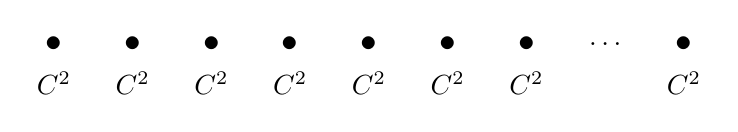
\begin{tikzpicture}
			\foreach \a in {0,1,...,6}{
				\node at (\a,0) {\large $\bullet$};	
			}
			\node at (7,0) {$\dots$};
			\node at (8,0) {\large $\bullet$};
			\foreach \a in {0,1,...,6}{
				\node at (\a,-0.5) {$\mathbb{C}^2$};	
			}
			\node at (8,-0.5) {$\mathbb{C}^2$};
		\end{tikzpicture}
	\end{equation}
Since the Hilbert space of a composite system is given by the tensor product of the individual Hilbert spaces, the total Hilbert space of a chain of $N$ spins is
	\begin{equation}
		\mathcal{H}_0=\bigotimes_{i=1}^N\mathbb{C}^2.
	\end{equation}

We now introduce defects to the chain, i.e., particles that behave differently than the spin-up/spin-down particles that are represented by the black bullets above. We begin by putting a single defect, indicated in red, at position $j$ in the chain:
	\begin{equation}
		\begin{tikzpicture}
			\foreach \a in {0,1,2,4,5,6}{
				\node at (\a,0) {\large $\bullet$};	
			}
			\node at (7,0) {$\dots$};
			\node at (3,0) {\large \color{LinkColor} $\bullet$};	
			\node at (8,0) {\large $\bullet$};
			\foreach \a in {0,1,2,4,5,6}{
				\node at (\a,-0.5) {$\mathbb{C}^2$};	
			}
			\node at (8,-0.5) {$\mathbb{C}^2$};
		\end{tikzpicture}
	\end{equation}
The defect can be anything that behaves differently than the particles of the chain, for example a particle with no spin. In this example, there is only one state this particle can be in (the ``no spin'' state), hence the corresponding Hilbert space is $\mathbb{C}$. As a result, the total Hilbert space $\mathcal{H}_1$ of a chain with one defect only differs to $\mathcal{H}_0$ at position $j$, where $\mathbb{C}^2$ is replaced by $\mathbb{C}$:
	\begin{equation}
		\mathcal{H}_1^{(j)}=\left(\bigotimes_{i=1}^{j-1}\mathbb{C}^2\right)\otimes\mathbb{C}\otimes\left(\bigotimes_{i=j+1}^{N}\mathbb{C}^2\right),
	\end{equation}
where the subscript describes the number of defects in the chain and the superscript indicates the position of the defect. It is also possible to consider both possibilities together, having no defect and having a defect at position $j$. This is described by the direct sum of the two Hilbert spaces:
	\begin{equation}
		\Hi=\Hi_0\oplus\Hi_1^{(j)}.
 	\end{equation}
We can generalize this model one step further by not specifying the position of the defect, i.e., allowing the defect to move. In this case, we get an additional sum over all positions $j$:
	\begin{equation}
		\Hi=\Hi_0\oplus\left(\bigoplus_{j=1}^N\Hi_1^{(j)}\right).
	\end{equation}
The above Hilbert space is the most general one for a chain with at most one defect. We can go one step further and allow \emph{two} defects in the chain, say at positions $j$ and $k$:
	\begin{equation}
		\begin{tikzpicture}
			\foreach \a in {0,1,2,4,6}{
				\node at (\a,0) {\large $\bullet$};	
			}
			\node at (7,0) {$\dots$};
			\node at (3,0) {\large \color{LinkColor} $\bullet$};	
			\node at (5,0) {\large \color{LinkColor} $\bullet$};
			\node at (8,0) {\large $\bullet$};
			\foreach \a in {0,1,2,4,6}{
				\node at (\a,-0.5) {$\mathbb{C}^2$};	
			}
			\node at (8,-0.5) {$\mathbb{C}^2$};
		\end{tikzpicture}
	\end{equation}
Similar to the description of a single defect, the Hilbert space of a chain with two defects is given by
	\begin{equation}
		\Hi_2^{(j,k)}=\left(\bigotimes_{i=1}^{j-1}\mathbb{C}^2\right)\otimes\mathbb{C}\otimes\left(\bigotimes_{i=j+1}^{k-1}\mathbb{C}^2\right)\otimes\mathbb{C}\otimes\left(\bigotimes_{i=k+1}^{N}\mathbb{C}^2\right).
	\end{equation}
Analogous to the single-defect case we allow the defects to move and, furthermore, we include the case of having either a single defect or no defect at all. This gives the Hilbert space for a spin chain with \emph{at most} two defects:
	\begin{equation}
		\Hi=\Hi_0\oplus\left(\bigoplus_{j=1}^N\Hi_1^{(j)}\right)\oplus\left(\bigoplus_{j=1}^N\bigoplus_{k\neq j}\Hi_2^{(j,k)}\right).
	\end{equation}
This procedure can be expanded to an arbitrary number of defects in the chain until we have a defect at every position. The Hilbert space in this case is simply $\Hi_N=\bigoplus_{i=1}^N\mathbb{C}$. Finally, we can define the Hilbert space of a chain of $n$ particles with an indefinite\footnote{Since the chain has only $N$ particles, the number of defects is naturally limited to a maximum of $N$.} number of defects that are allowed to move: 
	\begin{equation}
	\label{eq:Hilbertall}
		\Hi=\bigoplus_{n=\#\mathrm{ defects}}\Hi_n,
	\end{equation}
where 
	\begin{equation}
		\Hi_n\equiv\bigoplus_{j=1}^N\bigoplus_{k_1\neq j}\bigoplus_{k_2\neq k_1,j}\dots\bigoplus_{k_n\neq k_1,k_2,\dots,j}\Hi_n^{(j,k_1,k_2,\dots,k_n)}.
	\end{equation}
This Hilbert space is, unfortunately, highly complicated and therefore difficult to work with. However, there is a simpler way to describe it: At each site, the particle can be in one of three states: spin up, spin down, or no spin. Hence, we effectively have a three-level system at each site of the chain and the overall Hilbert space described in \cref{eq:Hilbertall} can be written as
	\begin{equation}
	\label{eq:totalHilb}
		\Hi\cong\bigotimes_{j=1}^N\left(\mathbb{C}\oplus\mathbb{C}^2\right)
	\end{equation}
which is much simpler than the previous expression. This description will be helpful in the following chapters when we study an explicit example of a spin chain with defects, namely a chain built from objects of the $\mathbf{Vec}(\mathbb{Z}/2\mathbb{Z})$ fusion category.


\section{A $\mathbf{Vec}(\mathbb{Z}/2\mathbb{Z})$ spin chain}

The spin chain introduced in the previous section and especially the effects of adding defects to it can be described via the fusion category $\mathbf{Vec}(\mathbb{Z}/2\mathbb{Z})$. First, remember that $\mathbf{Vec}(\mathbb{Z}/2\mathbb{Z})$ has two simple objects: $\Obj(\mathbf{Vec}(\mathbb{Z}/2\mathbb{Z}))=\{0,1\}$, where the vacuum is denoted $0$\footnote{Here, we do not follow our convention of denoting the vacuum $\mathbf{1}$ for convenience to be able to state the fusion rules as addition modulo $2$.} and $1$ is the non-trivial simple object in the category. The fusion rules are given by addition modulo 2, which results in the following fusion table:
	{{\setlength{\tabcolsep}{10pt}
			\renewcommand{\arraystretch}{1.25}
	\begin{table}[H]
		\centering
		\begin{tabular}{c||c|c}
			& 0 & 1 \\\hline\hline
			0 & 0 & 1 \\\hline
			1 & 1 & 0
		\end{tabular}
	\end{table}}
\noindent
Furthermore, the $F$-symbols of the category are trivial.

Let us now study the Hilbert space of the spin chain constructed from $\mathbf{Vec}(\mathbb{Z}/2\mathbb{Z})$\index{Vec(Z/2Z) chain@$\mathbf{Vec}(\mathbb{Z}/2\mathbb{Z})$ chain}. The choice of basis vectors here is very restricted. Suppose we set $a=1$. The resulting chain is\footnote{Note that we have not set the leftmost and the rightmost label to $a=1$ here, but included them into the labels of the basis state.} 
	\begin{figure}[H]
		\centering
		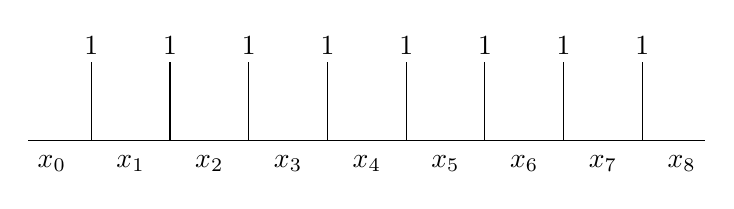
\begin{tikzpicture}[scale=2]
			\draw (0.1,0) -- (4.4,0);
			\draw (0.5,0) -- (0.5,0.5);
			\draw (1,0) -- (1,0.5);
			\draw (1.5,0) -- (1.5,0.5);
			\draw (2,0) -- (2,0.5);
			\draw (2.5,0) -- (2.5,0.5);
			\draw (3,0) -- (3,0.5);
			\draw (3.5,0) -- (3.5,0.5);
			\draw (4,0) -- (4,0.5);
			\node at (0.5,0.6) {$1$};
			\node at (1,0.6) {$1$};
			\node at (1.5,0.6) {$1$};
			\node at (2,0.6) {$1$};
			\node at (2.5,0.6) {$1$};
			\node at (3,0.6) {$1$};
			\node at (3.5,0.6) {$1$};
			\node at (4,0.6) {$1$};
			\node at (0.25,-0.15) {$x_0$};
			\node at (0.75,-0.15) {$x_1$};
			\node at (1.25,-0.15) {$x_2$};
			\node at (1.75,-0.15) {$x_3$};
			\node at (2.25,-0.15) {$x_4$};
			\node at (2.75,-0.15) {$x_5$};
			\node at (3.25,-0.15) {$x_6$};
			\node at (3.75,-0.15) {$x_7$};
			\node at (4.25,-0.15) {$x_8$};
		\end{tikzpicture}
	\end{figure}

There are only two possible basis states for the chain depicted above: $|1,0,1,0,1,0,1,0\rangle$ and $|0,1,0,1,0,1,0,1\rangle$. This is in fact true for any chain of this form, independent of its length, because the fusion rules demand that the $x_i$ are alternating labels. The situation is similar if we set $a=0$. The two possible basis state are (independent of the length of the chain) $|0,0,0,0,\dots\rangle$ and $|1,1,1,1,\dots\rangle$. Hence, for a fixed label $a$, we can interpret the Hilbert space of the chain as that of a qubit, which is $\mathbb{C}^2.$

This situation changes once we allow defects to fuse with the chain. Since the objects in the chain are elements of the category $\mathbf{Vec}(\mathbb{Z}/2\mathbb{Z})$, defects are $\mathbf{Vec}(\mathbb{Z}/2\mathbb{Z})$--$\mathbf{Vec}(\mathbb{Z}/2\mathbb{Z})$ bimodules. In the model we describe here we need the vacuum to occur in the fusion of two defects, which requires that the bimodule we use is invertible. 
Therefore, from the bimodules we have presented in \cref{ex:Vecbimod} we choose the invertible bimodule $F_1$ to model the defects. Recall that $F_1$ has only one simple object, so we generally omit writing a label for the bimodule object but indicate it with a red line. If it is helpful to use a label, we denote it \textasteriskcentered. 

Introducing one defect to the chain as depicted in \cref{fig:defect} does not change the dimension of the Hilbert space. The basis states are still determined by the labels on the boundary. However, fusing more than one defect to the chain opens up new possibilities: Consider a chain with two defects:

	\begin{figure}[H]
		\centering
		\begin{tikzpicture}[scale=2]
			\draw (0.1,0) -- (4.4,0);
			\draw (0.5,0) -- (0.5,0.5);
			\draw (1,0) -- (1,0.5);
			\draw (1.5,0) -- (1.5,0.5);
			\draw[very thick, LinkColor] (2,0) -- (2,0.5);
			\draw (2.5,0) -- (2.5,0.5);
			\draw (3,0) -- (3,0.5);
			\draw[very thick, LinkColor] (3.5,0) -- (3.5,0.5);
			\draw (4,0) -- (4,0.5);
			\node at (0.5,0.6) {$a$};
			\node at (1,0.6) {$a$};
			\node at (1.5,0.6) {$a$};
			\node at (2,0.6) {};
			\node at (2.5,0.6) {$a$};
			\node at (3,0.6) {$a$};
			\node at (3.5,0.6) {};
			\node at (4,0.6) {$a$};
			\node at (0.25,-0.15) {$\bullet$};
			\node at (0.75,-0.15) {$\bullet$};
			\node at (1.25,-0.15) {$\bullet$};
			\node at (1.75,-0.15) {$\bullet$};
			\node at (2.25,-0.15) {\color{LinkColor}$\bullet$};
			\node at (2.75,-0.15) {\color{LinkColor}$\bullet$};
			\node at (3.25,-0.15) {\color{LinkColor}$\bullet$};
			\node at (3.75,-0.15) {$\bullet$};
			\node at (4.25,-0.15) {$\bullet$};
		\end{tikzpicture}
	\end{figure}
\noindent
Here, the bullets between the two defects (indicated in red) are not determined by the outer labels of the chain since, in general, all of the following vertices are possible:
	\begin{figure}[H]
		\centering
		\begin{tikzpicture}[scale=1.5]
			\draw (0.1,0) -- (0.9,0);
			\draw[very thick, LinkColor] (0.5,0) -- (0.5,0.5);
			\node at (0.25,-0.15) {\small $0$};
			\node at (0.75,-0.15) {\small $0$};
			\begin{scope}[xshift=1.5cm]
				\draw (0.1,0) -- (0.9,0);
				\draw[very thick, LinkColor] (0.5,0) -- (0.5,0.5);
				\node at (0.25,-0.15) {\small $0$};
				\node at (0.75,-0.15) {\small $1$};
			\end{scope}
			\begin{scope}[xshift=3cm]
				\draw (0.1,0) -- (0.9,0);
				\draw[very thick, LinkColor] (0.5,0) -- (0.5,0.5);
				\node at (0.25,-0.15) {\small $1$};
				\node at (0.75,-0.15) {\small $0$};
			\end{scope}
			\begin{scope}[xshift=4.5cm]
				\draw (0.1,0) -- (0.9,0);
				\draw[very thick, LinkColor] (0.5,0) -- (0.5,0.5);
				\node at (0.25,-0.15) {\small $1$};
				\node at (0.75,-0.15) {\small $1$};
			\end{scope}
		\end{tikzpicture}
	\end{figure}

Note that once we fix one of the objects represented by the red bullets in the above chain, the fusion rules determine the values of the remaining red bullets, independent of the number of bullets. 
%Since there are two possible choices, $0$ and $1$, introducing two defects to the chain adds two states to the basis of the chain, which means that the Hilbert space is now that of two qubits. In general, the number of qubits that the chain represents is \#defects$-1$.
Additional to fusing defects to the chain we can also allow objects from the bimodule to live on the horizontal lines of the chain, i.e., the labels $x_i$ are not only simple objects of the category $\mathbf{Vec}(\mathbb{Z}/2\mathbb{Z})$ but also of the bimodule $F_1$. Consider this situation in a chain where \emph{only} defects are fused to the chain, which is of the form
	\begin{figure}[H]
		\centering
		\begin{tikzpicture}[scale=2]
			\draw[very thick, LinkColor] (0.5,0) -- (0.5,0.5);
			\draw[very thick, LinkColor] (1,0) -- (1,0.5);
			\draw[very thick, LinkColor] (1.5,0) -- (1.5,0.5);
			\draw[very thick, LinkColor] (2,0) -- (2,0.5);
			\draw[very thick, LinkColor] (2.5,0) -- (2.5,0.5);
			\draw[very thick, LinkColor] (3,0) -- (3,0.5);
			\draw[very thick, LinkColor] (3.5,0) -- (3.5,0.5);
			\draw[very thick, LinkColor] (4,0) -- (4,0.5);
			\draw[very thick,LinkColor2] (0.1,0) -- (4.4,0);
		\end{tikzpicture}
	\end{figure}
\noindent
with
	\begin{equation}
		\begin{tikzpicture}[baseline={([yshift=-3pt]current bounding box.center)}]
			\draw[very thick,LinkColor2] (0,0) -- (1,0);
		\end{tikzpicture}=
		\begin{tikzpicture}[baseline={([yshift=-3pt]current bounding box.center)}]
			\draw (0,0) -- (1,0);
		\end{tikzpicture}\oplus
		\begin{tikzpicture}[baseline={([yshift=-3pt]current bounding box.center)}]
			\draw[very thick,LinkColor] (0,0) -- (1,0);
		\end{tikzpicture},
	\end{equation}
which means that an object living on a blue line can either be from the category $\mathbf{Vec}(\mathbb{Z}/2\mathbb{Z})$ (black line), which is $0$ or $1$, or from the bimodule $F_1$ (red line), which can only be \textasteriskcentered. This implies that, according to the discussion in \cref{sec:Hilbertspace}, the Hilbert space that corresponds to an orange line is $\mathbb{C}^2\oplus\mathbb{C}\cong\mathbb{C}^3$. Hence, valid configurations of the chain are of the form
	\begin{equation}
	\label{eq:defectstates}
		\begin{tikzpicture}[scale=2,baseline={([yshift=-3pt]current bounding box.center)}]
			\draw[very thick, LinkColor] (0.5,0) -- (0.5,0.5);
			\draw[very thick, LinkColor] (1,0) -- (1,0.5);
			\draw[very thick, LinkColor] (1.5,0) -- (1.5,0.5);
			\draw[very thick, LinkColor] (2,0) -- (2,0.5);
			\draw[very thick, LinkColor] (2.5,0) -- (2.5,0.5);
			\draw[very thick, LinkColor] (3,0) -- (3,0.5);
			\draw[very thick, LinkColor] (3.5,0) -- (3.5,0.5);
			\draw[very thick, LinkColor] (4,0) -- (4,0.5);
			\draw (0.1,0) -- (4.4,0);
			\draw[very thick, LinkColor] (0.49,0) -- (1.01,0);
			\draw[very thick, LinkColor] (1.49,0) -- (2.01,0);
			\draw[very thick, LinkColor] (2.49,0) -- (3.01,0);
			\draw[very thick, LinkColor] (3.49,0) -- (4.01,0);
			\node at (0.25,-0.15) {$\mathbb{C}^2$};
			\node at (1.25,-0.15) {$\mathbb{C}^2$};
			\node at (2.25,-0.15) {$\mathbb{C}^2$};
			\node at (3.25,-0.15) {$\mathbb{C}^2$};
			\node at (4.25,-0.15) {$\mathbb{C}^2$};
		\end{tikzpicture}
	\end{equation}

The vertices that appear in the above chain are part of the data of the bimodule, see \cref{ex:Vecbimod}. However, a new vertex appears when introducing dynamics to the system. The Hamiltonian we consider is of the same form as the one for the golden chain defined in \cref{eq:localham}, i.e., fusion to the vacuum object $0$ is energetically favoured by assigning an energy of $-1$ to it. The full Hamiltonian is then given by
	\begin{equation}
	\label{eq:defectham}
		H=-\sum_i\frac{1}{\sqrt{2}} 
		\begin{tikzpicture}[baseline={([yshift=-3pt]current bounding box.center)}]
			\draw (0,0) to node[right] {\small $0$} (0,0.5);
			\draw[very thick, LinkColor] (0,0) -- (-0.5,-0.5);
			\draw[very thick, LinkColor] (0,0) -- (0.5,-0.5);
			\draw[very thick, LinkColor] (0,0.5) -- (-0.5,1);
			\draw[very thick, LinkColor] (0,0.5) -- (0.5,1);
		\end{tikzpicture},
	\end{equation}
where the normalization factor results from the fact that $\dim(\mathrm{\textasteriskcentered})=\sqrt{2}$. This Hamiltonian includes the vertex
	\begin{equation}
	\label{eq:bmvertex}
		\begin{tikzpicture}[scale=1,baseline={([yshift=-3pt]current bounding box.center)}]
			\draw[very thick, LinkColor] (0,0) -- (-0.5,-0.5);
			\draw[very thick, LinkColor] (0,0) -- (0.5,-0.5);
			\draw (0,0) -- (0,0.6);
		\end{tikzpicture},
	\end{equation}
which is neither defined in the category $\mathbf{Vec}(\mathbb{Z}/2\mathbb{Z})$ nor in the bimodule $F_1$. Hence, in order to study the action of the Hamiltonian in \cref{eq:defectham} on the chain we need to construct this vertex. In other words, our objective is to build the extended category $\mathbf{Vec}(\mathbb{Z}/2\mathbb{Z})\oplus F_1$.


\subsection*{Construction of the extended category}

To compute the vertex in \cref{eq:bmvertex} we need to construct a basis for the corresponding morphism space for each choice of labels on the vertex. Here, we utilize the so-called \emph{annular category}.

	\begin{defn}[Three-string annular category]
		Let $\mathcal{A}$, $\mathcal{B}$, and $\mathcal{C}$ be fusion categories and $\mathcal{M}$ an $(\mathcal{A},\mathcal{B})$ bimodule, $\mathcal{N}$ a $(\mathcal{B},\mathcal{C})$ bimodule, and $\mathcal{P}$ an $(\mathcal{A},\mathcal{C})$ bimodule. The three-string annular category\index{annular category} $\mathbf{Ann}_{\mathcal{M},\mathcal{N};\mathcal{P}}(\mathcal{A},\mathcal{B},\mathcal{C})$ is defined as follows: Simple objects are triplets $(m,n;p)\in\mathcal{M}\times\mathcal{N}\times\mathcal{P}$. The basis for a morphism space $(m,n;p)\to(m',n';p')$ is given by valid diagrams on the annulus (up to isotopy and local relations), i.e., diagrams of the form
			\begin{equation}
			\label{eq:annbasis}
				\begin{tikzpicture}[scale=1.2,baseline={([yshift=-3pt]current bounding box.center)}]
					\draw[dashed] (0,0) circle (0.5cm);
					\draw[dashed] (0,0) circle (1.6cm);
					\draw[LinkColor3, very thick] (-60:0.5) -- (-60:1.6);
					\draw[LinkColor2, very thick] (-120:0.5) -- (-120:1.6);
					\draw ([shift=(-60:1cm)]0,0) arc (-60:90:1cm);
					\draw ([shift=(-120:1.15cm)]0,0) arc (-120:-60:1.15cm);
					\draw ([shift=(240:0.85cm)]0,0) arc (240:90:0.85cm);
					\draw[LinkColor,very thick] (90:0.5) -- (90:1.6);
					\node at (90:.3cm){\small $p$};
					\node at (90:1.8cm){\small $p'$};
					\node at (-60:.3cm){\small $n$};
					\node at (-60:1.8cm){\small $n'$};
					\node at (-120:.3cm){\small $m$};
					\node at (-120:1.8cm){\small $m'$};
					\node at (-1,0.3) {\small $a$};
					\node at (1.15,0.3) {\small $c$};
					\node at (0,-1.3) {\small $b$};
				\end{tikzpicture}\ .
			\end{equation}
		For two morphisms $f:(m,n;p)\to(m',n';p')$ and $g:(m',n';p')\to(m'',n'';p'')$, the composition $g\circ f$ corresponds to drawing the diagram $g$ outside of the diagram $f$: 
			\begin{equation}
				\begin{tikzpicture}[scale=1.1,baseline={([yshift=-3pt]current bounding box.center)}]
					\draw[dashed, gray, thick, fill=gray!30!white] (0,0) circle (1.6cm);
					\draw[dashed] (0,0) circle (0.5cm);
					\draw[dashed] (0,0) circle (2.8cm);
					\draw[LinkColor3, very thick] (-60:0.5) -- (-60:2.8);
					\draw[LinkColor2, very thick] (-120:0.5) -- (-120:2.8);
					\draw ([shift=(-60:1cm)]0,0) arc (-60:90:1cm);
					\draw ([shift=(-60:2.25cm)]0,0) arc (-60:90:2.25cm);
					\draw ([shift=(-120:1.15cm)]0,0) arc (-120:-60:1.15cm);
					\draw ([shift=(240:0.85cm)]0,0) arc (240:90:0.85cm);
					\draw ([shift=(240:2.1cm)]0,0) arc (240:90:2.1cm);
					\draw ([shift=(-120:2.4cm)]0,0) arc (-120:-60:2.4cm);
					\draw[LinkColor,very thick] (90:0.5) -- (90:2.8);
					\node at (90:.3cm){\small $p$};
					\node at (100:1.85cm){\small $p'$};
					\node at (90:3.05cm){\small $p''$};
					\node at (-60:.3cm){\small $n$};
					\node at (-50:1.85cm){\small $n'$};
					\node at (-60:3.05cm){\small $n''$};
					\node at (-120:.3cm){\small $m$};
					\node at (-130:1.85cm){\small $m'$};
					\node at (-120:3.05cm){\small $m''$};
					\node at (-1,0.3) {\small $a$};
					\node at (1.15,0.3) {\small $c$};
					\node at (0,-1.3) {\small $b$};
					\node at (150:2.3) {\small $a'$};
					\node at (270:2.6) {\small $b'$};
					\node at (30:2.45) {\small $c'$};
				\end{tikzpicture}\ ,
			\end{equation}
		after which, isotopy and the $F$-symbols of the respective fusion categories can be used to reduce the diagram to a sum of diagrams of the form \cref{eq:annbasis}.
	\end{defn}


Note that it is possible to define $n$-string annular categories analogously. Two common examples are the one-string annular category with the string labelled by objects from the category itself, which is known as the \emph{tube algebra}\index{tube algebra} \cite{Ocneanu1994,Evans1995,Evans1998}, and the one-string annular category with the string labelled by an invertible bimodule, which is called \emph{dube algebra}\index{dube algebra} \cite{Williamson2017}. However, for the purpose of constructing bimodule vertices we only need the three-string annular category. The objective in our case is to find representations of the three-string annular category with bimodules $\mathcal{M}=\mathcal{N}=F_1$ and $\mathcal{P}=\mathbf{Vec}(\mathbb{Z}/2\mathbb{Z})$. In the following, we use the notation $\mathbf{Vec}_{\mathbb{Z}_2}$ instead of $\mathbf{Vec}(\mathbb{Z}/2\mathbb{Z})$ for clarity and omit drawing the outer circle of the diagram in \cref{eq:annbasis}. 

To construct vertices in the extended category $\mathbf{Vec}_{\mathbb{Z}_2}$ we use the so-called ``inflation trick'' that was developed in \cite{Bridgeman2019,Bridgeman2020a,Bridgeman2020b}. This is a technique to construct representations of the annular category using primitive idempotents of the category. In our example, we need representations of morphisms in the annular category $\mathbf{Ann}_{F_1,F_1;\mathbf{Vec}_{\mathbb{Z}_2}}(\mathbf{Vec}_{\mathbb{Z}_2},\mathbf{Vec}_{\mathbb{Z}_2},\mathbf{Vec}_{\mathbb{Z}_2})$. More precisely, our goal it to find a basis for each vertex in the extended category $\mathbf{Vec}_{\mathbb{Z}_2}\oplus F_1$ (that is not determined either in $\mathbf{Vec}_{\mathbb{Z}_2}$ or in $F_1$) in terms of annular diagrams. In the following, we explicitly show step-by-step how the vertex in \cref{eq:bmvertex} is constructed using this technique.


\subsection*{Step 1: Compute isomorphism classes of simple objects}

The first step is to identify the isomorphism classes of simple objects in the category and pick a representative for each class. For the category $\mathbf{Ann}_{F_1,F_1;\mathbf{Vec}_{\mathbb{Z}_2}}(\mathbf{Vec}_{\mathbb{Z}_2},\mathbf{Vec}_{\mathbb{Z}_2},\mathbf{Vec}_{\mathbb{Z}_2})$, simple objects are of the form $(\mathrm{\textasteriskcentered},\mathrm{\textasteriskcentered},a)$, hence morphisms are given by diagrams of the form
	\begin{equation}
		\begin{tikzpicture}[scale=1.2,baseline={([yshift=-3pt]current bounding box.center)}]
			\draw (0,0) circle (0.5cm);
			\draw[LinkColor, very thick] (-60:0.5) -- (-60:1.6);
			\draw[LinkColor, very thick] (-120:0.5) -- (-120:1.6);
			\draw ([shift=(-60:1cm)]0,0) arc (-60:90:1cm);
			\draw ([shift=(-120:1.15cm)]0,0) arc (-120:-60:1.15cm);
			\draw ([shift=(240:0.85cm)]0,0) arc (240:90:0.85cm);
			\draw (90:0.5) -- (90:1.6);
			\node at (90:.3cm){\small $a$};
			\node at (90:1.8cm){\small $a+x+z$};
			\node at (-60:.3cm){};
			\node at (-60:1.8cm){};
			\node at (-120:.3cm){};
			\node at (-120:1.8cm){};
			\node at (-1,0.3) {\small $x$};
			\node at (1.15,0.3) {\small $z$};
			\node at (0,-1.3) {\small $y$};
		\end{tikzpicture}\ .
	\end{equation}
Since any morphism between simple objects is an isomorphism, the figure above implies that $(\mathrm{\textasteriskcentered},\mathrm{\textasteriskcentered},a)\cong(\mathrm{\textasteriskcentered},\mathrm{\textasteriskcentered},a+x+z)$ for all possible labels $x,y,z\in\mathbf{Vec}_{\mathbb{Z}_2}$. Hence, there is only one isomorphism class of simple objects and we pick $(\mathrm{\textasteriskcentered},\mathrm{\textasteriskcentered},0)$ as its representative.


\subsection*{Step 2: Find primitive idempotents}

To find a representation of the annular category, we need to find the simple objects in the \emph{Karoubi envelope} (see \cite{barter_domain_2019} for an explanation of this technique). This can be done by constructing the primitive idempotents. In the following, we use the notation $T_iT_j\equiv T_i\circ T_j$.
%\todo[inline]{Why do primitive idempotents give a representation of the category?}
	\begin{defn}
		A set of primitive idempotents\index{primitive idempotent} is a set of morphisms $\{T_i\}$ which fulfil
			\begin{align}
				T_iT_i&=T_i,\\
				T_iT_j&=0,\\
				T_i&\neq \sum_jf_j,
			\end{align}
		where the $f_j$ are (not necessarily primitive) idempotents, i.e., $f_jf_j=f_j$.
	\end{defn}

This means that we need to find morphisms $T: (\mathrm{\textasteriskcentered},\mathrm{\textasteriskcentered},0)\to(\mathrm{\textasteriskcentered},\mathrm{\textasteriskcentered},0)$ which square to themselves and are orthogonal to each other. Since we furthermore look for \emph{primitive} idempotents, it is also essential that they cannot be written as a sum of idempotents. Candidates for these idempotents are those morphisms where $x+z=0$, since otherwise it is not possible to compose $T$ with itself. Therefore, a morphism is labelled by the two labels $x$ and $y$, hence there are four possible candidates $T_{x,y}$ (note that we do not draw lines when $x,y,z$ are the vacuum object $0$):
	\begin{align}
		T_{0,0}=
		\begin{tikzpicture}[scale=0.9,baseline={([yshift=-3pt]current bounding box.center)}]
			\draw (0,0) circle (0.5cm);
			\draw[LinkColor, very thick] (-60:0.5) -- (-60:1.6);
			\draw[LinkColor, very thick] (-120:0.5) -- (-120:1.6);
			\draw (90:0.5) -- (90:1.6);
			\node at (90:.25cm){\small $0$};
			\node at (90:1.8cm){\small $0$};
			\node at (-60:.3cm){};
			\node at (-60:1.8cm){};
			\node at (-120:.3cm){};
			\node at (-120:1.8cm){};
		\end{tikzpicture},\hspace{10pt}T_{0,1}=
		\begin{tikzpicture}[scale=0.9,baseline={([yshift=-3pt]current bounding box.center)}]
			\draw (0,0) circle (0.5cm);
			\draw[LinkColor, very thick] (-60:0.5) -- (-60:1.6);
			\draw[LinkColor, very thick] (-120:0.5) -- (-120:1.6);
			\draw (90:0.5) -- (90:1.6);
			\node at (90:.25cm){\small $0$};
			\node at (90:1.8cm){\small $0$};
			\node at (-60:.3cm){};
			\node at (-60:1.8cm){};
			\node at (-120:.3cm){};
			\node at (-120:1.8cm){};
			\draw ([shift=(-120:1.15cm)]0,0) arc (-120:-60:1.15cm);
			\node at (0,-1.35) {\small $1$};
		\end{tikzpicture},\hspace{10pt}
		T_{1,0}=
		\begin{tikzpicture}[scale=0.9,baseline={([yshift=-3pt]current bounding box.center)}]
			\draw (0,0) circle (0.5cm);
			\draw[LinkColor, very thick] (-60:0.5) -- (-60:1.6);
			\draw[LinkColor, very thick] (-120:0.5) -- (-120:1.6);
			\draw (90:0.5) -- (90:1.6);
			\node at (90:.25cm){\small $0$};
			\node at (90:1.8cm){\small $0$};
			\node at (-60:.3cm){};
			\node at (-60:1.8cm){};
			\node at (-120:.3cm){};
			\node at (-120:1.8cm){};
			\draw ([shift=(-60:1cm)]0,0) arc (-60:90:1cm);
			\draw ([shift=(240:0.85cm)]0,0) arc (240:90:0.85cm);
			\node at (-1,0.3) {\small $1$};
			\node at (1.15,0.3) {\small $1$};
		\end{tikzpicture},\hspace{10pt}T_{1,1}=
		\begin{tikzpicture}[scale=0.9,baseline={([yshift=-3pt]current bounding box.center)}]
			\draw (0,0) circle (0.5cm);
			\draw[LinkColor, very thick] (-60:0.5) -- (-60:1.6);
			\draw[LinkColor, very thick] (-120:0.5) -- (-120:1.6);
			\draw ([shift=(-60:1cm)]0,0) arc (-60:90:1cm);
			\draw ([shift=(-120:1.15cm)]0,0) arc (-120:-60:1.15cm);
			\draw ([shift=(240:0.85cm)]0,0) arc (240:90:0.85cm);
			\draw (90:0.5) -- (90:1.6);
			\node at (90:.25cm){\small $0$};
			\node at (90:1.8cm){\small $0$};
			\node at (-60:.3cm){};
			\node at (-60:1.8cm){};
			\node at (-120:.3cm){};
			\node at (-120:1.8cm){};
			\node at (-1,0.3) {\small $1$};
			\node at (1.15,0.3) {\small $1$};
			\node at (0,-1.35) {\small $1$};
		\end{tikzpicture}.
	\end{align}
	
The first morphism, $T_{0,0}$, can be interpreted as the identity morphism and it obviously squares to itself. $T_{0,1}^2$ and $T_{1,0}^2$ are computed as follows\footnote{Remember that the associator of the category $\mathbf{Vec}_{\mathbb{Z}_2}$ is trivial. Furthermore, the bimodule $F_1$ has a trivial left associator $L$ as a left module category and a trivial right associator $R$ as a right module category. Also, the dimension of all simple objects is one, so bubble popping does not introduce any factors.}:
	\begin{align}
		T_{0,1}^2=
		\begin{tikzpicture}[scale=0.9,baseline={([yshift=-3pt]current bounding box.center)}]
			\draw (0,0) circle (0.5cm);
			\draw[LinkColor, very thick]
			\foreach \a in {-60, -120} {
				(\a:0.5) -- (\a:2)
			};
			\draw[] (90:0.5) -- (90:2);
			\draw ([shift=(-120:1.15cm)]0,0) arc (-120:-60:1.15cm);
			\draw ([shift=(-120:1.6cm)]0,0) arc (-120:-60:1.6cm);
			\node at (90:.25cm){\small $0$};
			\node at (90:2.25cm){\small $0$};
			\node at (0,-1.35) {\small $1$};
			\node at (0,-1.8) {\small $1$};
		\end{tikzpicture}
		\ =\ \begin{tikzpicture}[scale=0.9,baseline={([yshift=-3pt]current bounding box.center)}]
			\draw (0,0) circle (0.5cm);
			\draw[LinkColor, very thick]
			\foreach \a in {-60, -120} {
				(\a:0.5) -- (\a:2)
			};
			\draw[] (90:0.5) -- (90:2);
			\draw ([shift=(-120:1.4cm)]0,0) arc (-120:-105:1.4cm);
%			\draw ([shift=(-120:1.6cm)]0,0) arc (-120:-105:1.6cm);
			\draw ([shift=(-75:1.4cm)]0,0) arc (-75:-60:1.4cm);
%			\draw ([shift=(-75:1.6cm)]0,0) arc (-75:-60:1.6cm);
			\draw (-105:1.4cm) to[bend right=80] (-75:1.4cm);
			\draw (-105:1.4cm) to[bend left=80] (-75:1.4cm);
			\node at (90:.25cm){\small $0$};
			\node at (90:2.25cm){\small $0$};
			\node at (0,-0.95) {\small $1$};
			\node at (0,-1.8) {\small $1$};
			\node at (0.55,-1.5) {\small $1$};
			\node at (-0.55,-1.5) {\small $1$};
		\end{tikzpicture}
		\ =\ \begin{tikzpicture}[scale=0.9,baseline={([yshift=-3pt]current bounding box.center)}]
			\draw (0,0) circle (0.5cm);
			\draw[LinkColor, very thick] (-60:0.5) -- (-60:1.6);
			\draw[LinkColor, very thick] (-120:0.5) -- (-120:1.6);
			\draw (90:0.5) -- (90:1.6);
			\node at (90:.25cm){\small $0$};
			\node at (90:1.8cm){\small $0$};
			\node at (-60:.3cm){};
			\node at (-60:1.8cm){};
			\node at (-120:.3cm){};
			\node at (-120:1.8cm){};
		\end{tikzpicture},
	\end{align}
	\begin{align}
		T_{1,0}^2=
		\begin{tikzpicture}[scale=0.9,baseline={([yshift=-3pt]current bounding box.center)}]
			\draw (0,0) circle (0.5cm);
			\draw[LinkColor, very thick]
			\foreach \a in {-60, -120} {
				(\a:0.5) -- (\a:2)
			};
			\draw[] (90:0.5) -- (90:2);
			\draw ([shift=(-60:1cm)]0,0) arc (-60:90:1cm);
			\draw ([shift=(240:0.85cm)]0,0) arc (240:90:0.85cm);
			\draw ([shift=(240:1.3cm)]0,0) arc (240:90:1.3cm);
			\draw ([shift=(-60:1.45cm)]0,0) arc (-60:90:1.45cm);
			\node at (90:.25cm){\small $0$};
			\node at (90:2.25cm){\small $0$};
			\node at (-1,0.3) {\small $1$};
			\node at (1.15,0.3) {\small $1$};
			\node at (-1.4,0.6) {\small $1$};
			\node at (1.5,0.6) {\small $1$};
			\end{tikzpicture}
		=\begin{tikzpicture}[scale=0.9,baseline={([yshift=-3pt]current bounding box.center)}]
			\draw (0,0) circle (0.5cm);
			\draw[LinkColor, very thick]
			\foreach \a in {-60, -120} {
				(\a:0.5) -- (\a:2)
			};
			\draw[] (90:0.5) -- (90:2);
			\draw ([shift=(240:0.75cm)]0,0) arc (240:90:0.75cm);
			\draw ([shift=(-60:1cm)]0,0) to [bend right=70] ([shift=(90:1.4cm)]0,0);
			\draw ([shift=(240:1.1cm)]0,0) arc (240:90:1.1cm);
			\draw ([shift=(-60:1.4cm)]0,0) to [bend right=70] ([shift=(90:1.75cm)]0,0);
			\node at (90:.25cm){\small $0$};
			\node at (90:2.25cm){\small $0$};
			\node at (-0.9,0.3) {\small $1$};
			\node at (1.05,0.3) {\small $1$};
			\node at (-1.2,0.6) {\small $1$};
			\node at (1.35,0.6) {\small $1$};
		\end{tikzpicture}
		=\begin{tikzpicture}[scale=0.9,baseline={([yshift=-3pt]current bounding box.center)}]
			\draw (0,0) circle (0.5cm);
			\draw[LinkColor, very thick] (-60:0.5) -- (-60:1.6);
			\draw[LinkColor, very thick] (-120:0.5) -- (-120:1.6);
			\draw (90:0.5) -- (90:1.6);
			\node at (90:.25cm){\small $0$};
			\node at (90:1.8cm){\small $0$};
			\node at (-60:.3cm){};
			\node at (-60:1.8cm){};
			\node at (-120:.3cm){};
			\node at (-120:1.8cm){};
		\end{tikzpicture}.
	\end{align}
so both of them do not square to themselves but to $T_{0,0}$. The calculation for the fourth candidate is a little more intricate, since this is the only one where the non-trivial associator of $F_1$ appears:
	\begin{align}
		\begin{tikzpicture}[scale=0.9,baseline={([yshift=-3pt]current bounding box.center)}]
			\draw (0,0) circle (0.5cm);
			\draw[LinkColor, very thick]
			\foreach \a in {-60, -120} {
				(\a:0.5) -- (\a:2)
			};
			\draw[] (90:0.5) -- (90:2);
			\draw ([shift=(-60:1cm)]0,0) arc (-60:90:1cm);
			\draw ([shift=(-120:1.15cm)]0,0) arc (-120:-60:1.15cm);
			\draw ([shift=(240:0.85cm)]0,0) arc (240:90:0.85cm);
			\draw ([shift=(240:1.3cm)]0,0) arc (240:90:1.3cm);
			\draw ([shift=(-60:1.45cm)]0,0) arc (-60:90:1.45cm);
			\draw ([shift=(-120:1.6cm)]0,0) arc (-120:-60:1.6cm);
			\node at (90:.25cm){\small $0$};
			\node at (90:2.25cm){\small $0$};
			\node at (-1,0.3) {\small $1$};
			\node at (1.15,0.3) {\small $1$};
			\node at (0,-1.35) {\small $1$};
			\node at (-1.4,0.6) {\small $1$};
			\node at (1.5,0.6) {\small $1$};
			\node at (0,-1.8) {\small $1$};
		\end{tikzpicture}
		=-\begin{tikzpicture}[scale=0.9,baseline={([yshift=-3pt]current bounding box.center)}]
			\draw (0,0) circle (0.5cm);
			\draw[LinkColor, very thick]
			\foreach \a in {-60, -120} {
				(\a:0.5) -- (\a:2)
			};
			\draw[] (90:0.5) -- (90:2);
			\draw ([shift=(-60:1cm)]0,0) arc (-60:90:1cm);
			\draw ([shift=(-120:1.25cm)]0,0) arc (-120:-60:1.25cm);
			\draw ([shift=(240:0.85cm)]0,0) arc (240:90:0.85cm);
			\draw ([shift=(240:1.15cm)]0,0) arc (240:90:1.15cm);
			\draw ([shift=(-60:1.45cm)]0,0) arc (-60:90:1.45cm);
			\draw ([shift=(-120:1.6cm)]0,0) arc (-120:-60:1.6cm);
			\node at (90:.25cm){\small $0$};
			\node at (90:2.25cm){\small $0$};
			\node at (-1.1,0.8) {\small $1$};
			\node at (1.15,0.3) {\small $1$};
			\node at (0,-1.4) {\small $1$};
			\node at (-0.8,0.6) {\small $1$};
			\node at (1.5,0.6) {\small $1$};
			\node at (0,-1.8) {\small $1$};
		\end{tikzpicture}
		=\begin{tikzpicture}[scale=0.9,baseline={([yshift=-3pt]current bounding box.center)}]
			\draw (0,0) circle (0.5cm);
			\draw[LinkColor, very thick]
			\foreach \a in {-60, -120} {
				(\a:0.5) -- (\a:2)
			};
			\draw[] (90:0.5) -- (90:2);
			\draw ([shift=(240:0.75cm)]0,0) arc (240:90:0.75cm);
			\draw ([shift=(-60:1cm)]0,0) to [bend right=70] ([shift=(90:1.4cm)]0,0);
			\draw ([shift=(-120:1.5cm)]0,0) arc (-120:-60:1.5cm);
			\draw ([shift=(240:1.1cm)]0,0) arc (240:90:1.1cm);
			\draw ([shift=(-60:1.4cm)]0,0) to [bend right=70] ([shift=(90:1.75cm)]0,0);
			\draw ([shift=(-120:1.8cm)]0,0) arc (-120:-60:1.8cm);
			\node at (90:.25cm){\small $0$};
			\node at (90:2.25cm){\small $0$};
			\node at (-0.9,0.3) {\small $1$};
			\node at (1.05,0.3) {\small $1$};
			\node at (0,-1.65) {\small $1$};
			\node at (-1.2,0.6) {\small $1$};
			\node at (1.35,0.6) {\small $1$};
			\node at (0,-2) {\small $1$};
		\end{tikzpicture}
		=\begin{tikzpicture}[scale=0.9,baseline={([yshift=-3pt]current bounding box.center)}]
				\draw (0,0) circle (0.5cm);
			\draw[LinkColor, very thick]
			\foreach \a in {-60, -120} {
				(\a:0.5) -- (\a:1.6)
			};
			\draw[] (90:0.5) -- (90:1.6);
			\node at (90:.25cm){\small $0$};
			\node at (90:1.75cm){\small $0$};
		\end{tikzpicture}.
	\end{align}
The first equality here follows from applying the non-trivial associator of the bimodule $F_1$, which introduces a negative sign to the diagram. As the previous candidates, $T_{1,1}$ also squares to $T_{0,0}$. Hence, none of these candidates is a primitive idempotent. In fact, similar computations show that the general multiplication rule for the $T_{i,j}$ is
	\begin{equation}
	\label{eq:multrule}
		T_{a,b}T_{c,d}=T_{a+c,b+d}.
	\end{equation} 
However, since we have four candidates $T_{i,j}$ for the primitive idempotents, we know that the algebra of primitive idempotents is four-dimensional. In an algebra, it is also possible to consider linear combinations of the candidates. To find suitable linear combinations of the candidates that form a primitive idempotent, it is helpful to work with matrices instead of diagrams on the annulus. More precisely, we need to construct a set of four-dimensional matrices that multiplies in the same way as the four candidates. Since we already know the primitive idempotents for four-dimensional matrices, we can then use these matrices to easily decompose them into primitive idempotents. 

The easiest diagram to translate into a matrix is $T_{0,0}$ since it is the identity. Therefore, the corresponding matrix is 
	\begin{equation}
		M_{0,0}=\begin{pmatrix}
			1 & 0 & 0 & 0\\
			0 & 1 & 0 & 0\\
			0 & 0 & 1 & 0\\
			0 & 0 & 0 & 1
		\end{pmatrix}.
	\end{equation}
We have already seen that it is an idempotent (it squares to itself), but it is not a primitive one since it can be written as a sum of matrices that square to themselves:
	\begin{equation}
	\label{eq:primi}
		M_{0,0}=\begin{pmatrix}
		1 & 0 & 0 & 0\\
		0 & 0 & 0 & 0\\
		0 & 0 & 0 & 0\\
		0 & 0 & 0 & 0
		\end{pmatrix}+\begin{pmatrix}
		0 & 0 & 0 & 0\\
		0 & 1 & 0 & 0\\
		0 & 0 & 0 & 0\\
		0 & 0 & 0 & 0
		\end{pmatrix}+\begin{pmatrix}
		0 & 0 & 0 & 0\\
		0 & 0 & 0 & 0\\
		0 & 0 & 1 & 0\\
		0 & 0 & 0 & 0
		\end{pmatrix}+\begin{pmatrix}
		0 & 0 & 0 & 0\\
		0 & 0 & 0 & 0\\
		0 & 0 & 0 & 0\\
		0 & 0 & 0 & 1
		\end{pmatrix}.
	\end{equation}
Since the matrix that represents the second candidate has to fulfil $M_{0,1}^2=M_{0,0}$ a possible candidate is
	\begin{equation}
		M_{0,1}=\begin{pmatrix}
		1 & 0 & 0 & 0\\
		0 & 1 & 0 & 0\\
		0 & 0 & -1 & 0\\
		0 & 0 & 0 & -1
		\end{pmatrix}.
	\end{equation}
Similar matrices can be found for the remaining two candidates:
	\begin{equation}
		M_{1,0}=\begin{pmatrix}
		-1 & 0 & 0 & 0\\
		0 & 1 & 0 & 0\\
		0 & 0 & -1 & 0\\
		0 & 0 & 0 & 1
		\end{pmatrix},\hspace{20pt}
		M_{1,1}=\begin{pmatrix}
		-1 & 0 & 0 & 0\\
		0 & 1 & 0 & 0\\
		0 & 0 & 1 & 0\\
		0 & 0 & 0 & -1
		\end{pmatrix}.
	\end{equation}
It is straightforward to check that the set of matrices $\{M_{i,j}\}$ fulfils the general multiplication rule for the four candidates \cref{eq:multrule}. We now need to express the four primitive idempotents from \cref{eq:primi} as linear combinations of the $M_{i,j}$ to be able to translate them back into annular diagrams. The general formula for a primitive idempotent is given by
	\begin{equation}
	\label{eq:primidem}
		P_{x,y}=\frac{1}{4}\sum_{a,b}(-1)^{ax+by}M_{a,b}.
	\end{equation}
In terms of annular diagrams, primitive idempotents are hence depicted
	\begin{align}
		P_{x,y}&=\frac{1}{4}\sum_{a,b}(-1)^{ax+by}\begin{tikzpicture}[scale=0.9,baseline={([yshift=-3pt]current bounding box.center)}]
			\draw (0,0) circle (0.5cm);
			\draw[LinkColor, very thick] (-60:0.5) -- (-60:1.6);
			\draw[LinkColor, very thick] (-120:0.5) -- (-120:1.6);
			\draw ([shift=(-60:1cm)]0,0) arc (-60:90:1cm);
			\draw ([shift=(-120:1.15cm)]0,0) arc (-120:-60:1.15cm);
			\draw ([shift=(240:0.85cm)]0,0) arc (240:90:0.85cm);
			\draw (90:0.5) -- (90:1.6);
			\node at (90:.25cm){\small $0$};
			\node at (90:1.8cm){\small $0$};
			\node at (-60:.3cm){};
			\node at (-60:1.8cm){};
			\node at (-120:.3cm){};
			\node at (-120:1.8cm){};
			\node at (-1,0.3) {\small $b$};
			\node at (1.15,0.3) {\small $b$};
			\node at (0,-1.35) {\small $a$};
		\end{tikzpicture}\\
		&=\frac{1}{4}\left(\begin{tikzpicture}[scale=0.9,baseline={([yshift=-3pt]current bounding box.center)}]
			\draw (0,0) circle (0.5cm);
			\draw[LinkColor, very thick] (-60:0.5) -- (-60:1.6);
			\draw[LinkColor, very thick] (-120:0.5) -- (-120:1.6);
			\draw (90:0.5) -- (90:1.6);
			\node at (90:.25cm){\small $0$};
			\node at (90:1.8cm){\small $0$};
			\node at (-60:.3cm){};
			\node at (-60:1.8cm){};
			\node at (-120:.3cm){};
			\node at (-120:1.8cm){};
		\end{tikzpicture}+(-1)^x
		\begin{tikzpicture}[scale=0.9,baseline={([yshift=-3pt]current bounding box.center)}]
			\draw (0,0) circle (0.5cm);
			\draw[LinkColor, very thick] (-60:0.5) -- (-60:1.6);
			\draw[LinkColor, very thick] (-120:0.5) -- (-120:1.6);
			\draw (90:0.5) -- (90:1.6);
			\node at (90:.25cm){\small $0$};
			\node at (90:1.8cm){\small $0$};
			\node at (-60:.3cm){};
			\node at (-60:1.8cm){};
			\node at (-120:.3cm){};
			\node at (-120:1.8cm){};
			\draw ([shift=(-120:1.15cm)]0,0) arc (-120:-60:1.15cm);
			\node at (0,-1.35) {\small $1$};
		\end{tikzpicture}+(-1)^y
		\begin{tikzpicture}[scale=0.9,baseline={([yshift=-3pt]current bounding box.center)}]
			\draw (0,0) circle (0.5cm);
			\draw[LinkColor, very thick] (-60:0.5) -- (-60:1.6);
			\draw[LinkColor, very thick] (-120:0.5) -- (-120:1.6);
			\draw (90:0.5) -- (90:1.6);
			\node at (90:.25cm){\small $0$};
			\node at (90:1.8cm){\small $0$};
			\node at (-60:.3cm){};
			\node at (-60:1.8cm){};
			\node at (-120:.3cm){};
			\node at (-120:1.8cm){};
			\draw ([shift=(-60:1cm)]0,0) arc (-60:90:1cm);
			\draw ([shift=(240:0.85cm)]0,0) arc (240:90:0.85cm);
			\node at (-1,0.3) {\small $1$};
			\node at (1.15,0.3) {\small $1$};
		\end{tikzpicture}+(-1)^{x+y}
		\begin{tikzpicture}[scale=0.9,baseline={([yshift=-3pt]current bounding box.center)}]
		\draw (0,0) circle (0.5cm);
			\draw[LinkColor, very thick] (-60:0.5) -- (-60:1.6);
			\draw[LinkColor, very thick] (-120:0.5) -- (-120:1.6);
			\draw ([shift=(-60:1cm)]0,0) arc (-60:90:1cm);
			\draw ([shift=(-120:1.15cm)]0,0) arc (-120:-60:1.15cm);
			\draw ([shift=(240:0.85cm)]0,0) arc (240:90:0.85cm);
			\draw (90:0.5) -- (90:1.6);
			\node at (90:.25cm){\small $0$};
			\node at (90:1.8cm){\small $0$};
			\node at (-60:.3cm){};
			\node at (-60:1.8cm){};
			\node at (-120:.3cm){};
			\node at (-120:1.8cm){};
			\node at (-1,0.3) {\small $1$};
			\node at (1.15,0.3) {\small $1$};
			\node at (0,-1.35) {\small $1$};
		\end{tikzpicture}
		\right).
	\end{align}


\subsection*{Step 3: Check for isomorphism classes of primitive idempotents}

In general, the primitive idempotents we have found in the previous step can be isomorphic to each other. In this case, we have to pick one representative for each isomorphism class. Two idempotents are isomorphic to each other if there are matrices within the algebra that can be multiplied to $P_{x,y}$ to get $P_{x',y'}$. For example, we can get $P_{1,0}$ from $P_{0,1}$ via 
	\begin{equation}
	\label{eq:isomP}
		\begin{pmatrix}
			0 & 0 & 0 & 0\\
			0 & 0 & 0 & 0\\
			0 & 1 & 0 & 0\\
			0 & 0 & 0 & 0
		\end{pmatrix}P_{0,1}
		\begin{pmatrix}
			0 & 0 & 0 & 0\\
			0 & 0 & 1 & 0\\
			0 & 0 & 0 & 0\\
			0 & 0 & 0 & 0
		\end{pmatrix}=P_{1,0}.
	\end{equation}
However, the matrices we used here are not elements of the matrix algebra since elements of the algebra only have entries on the diagonal. If the matrices were elements of the algebra then they would form an isomorphism between $P_{0,1}$ and $P_{1,0}$, hence we would pick one of them as a representative of the isomorphism class. However, in our case none of the four primitive idempotents are isomorphic to each other so we do not need to pick representatives, hence we find that there are four isomorphism classes.

In general, this step can me much more complicated if the algebra is higher-dimensional. Fortunately, there is a trick that helps us to see how many isomorphism classes there are, namely the \emph{Artin-Wedderburn theorem}\index{Artin-Wedderburn theorem}\index{Artin-Wedderburn theorem} (see for example \cite{Beachy1999}). It states that every semisimple matrix algebra is isomorphic to a finite direct sum of full matrix algebras, i.e.,
	\begin{equation}
		\mathcal{M}\cong \bigoplus\mathcal{M}_d
	\end{equation}
with $\dim\mathcal{M}_d=d^2$. For each full matrix algebra, we get exactly one primitive idempotent: We can, for example, pick the primitive idempotent $\mathrm{diag}(1,0,0,\dots)$. Every other primitive idempotent is isomorphic to this one since equations like \cref{eq:isomP} always exist within a \emph{full} matrix algebra. 

In our case, the algebra $\mathcal{M}$ is four-dimensional. The two possible decompositions into full matrix algebras are $\mathcal{M}\cong\mathbb{C}\oplus\mathbb{C}\oplus\mathbb{C}\oplus\mathbb{C}$ and $\mathcal{M}\cong\mathcal{M}_2(\mathbb{C})$. The first decomposition is the correct one since we have found four non-isomorphic primitive idempotents by the construction above. In case of a five-dimensional algebra $\mathcal{M}'$, for example, the two possible decompositions are $\mathcal{M}'\cong\mathbb{C}\oplus\mathcal{M}_2(\mathbb{C})$ and $\mathcal{M}'=\mathbb{C}\oplus\mathbb{C}\oplus\mathbb{C}\oplus\mathbb{C}\oplus\mathbb{C}$, hence there are either two or five primitive idempotents. These examples illustrate how using the Artin-Wedderburn theorem can make the task of determining the number of primitive idempotents much easier, since it drastically limits the number of possibilities.



\subsection*{Step 4: Build the full representation}

Remember that the goal of the whole calculation is to find a representation for the vertex
	\begin{equation}
		\begin{tikzpicture}[scale=1,baseline={([yshift=-3pt]current bounding box.center)}]
			\draw[very thick, LinkColor] (0,0) -- (-0.5,-0.5);
			\draw[very thick, LinkColor] (0,0) -- (0.5,-0.5);
			\draw (0,0) -- (0,0.6);
			\node at (0,0.75) {\small $x$};
		\end{tikzpicture},
	\end{equation}
with $x\in\{0,1\}$ in terms of annular diagrams. This corresponds to finding a basis for the morphism space $\Hom\big((\mathrm{\textasteriskcentered},\mathrm{\textasteriskcentered},0),(\mathrm{\textasteriskcentered},\mathrm{\textasteriskcentered},x)\big)$ for every possible $x$.

With the set of primitive idempotents at hand we can now build the full representation of the annular category, which is done by putting all possible annuli on the outside of the idempotents. This procedure allows us to find all basis vectors for the morphism spaces, i.e., all possible vectors of the form\footnote{Note that, in general, we would have to do this for every representative of an isomorphism class of simple objects, but in this example wo only have one.}
	\begin{equation}
	\label{eq:annulivec}
		\begin{tikzpicture}[scale=1.2,baseline={([yshift=-3pt]current bounding box.center)}]
			\draw (0,0) circle (0.5cm);
			\draw[LinkColor, very thick] (-60:0.5) -- (-60:1.6);
			\draw[LinkColor, very thick] (-120:0.5) -- (-120:1.6);
			\draw ([shift=(-60:1cm)]0,0) arc (-60:90:1cm);
			\draw ([shift=(-120:1.15cm)]0,0) arc (-120:-60:1.15cm);
			\draw ([shift=(240:0.85cm)]0,0) arc (240:90:0.85cm);
			\draw (90:0.5) -- (90:1.6);
			\node at (90:.3cm){\small $0$};
			\node at (90:1.8cm){\small $\alpha+\gamma$};
			\node at (-60:.3cm){};
			\node at (-60:1.8cm){};
			\node at (-120:.3cm){};
			\node at (-120:1.8cm){};
			\node at (-1,0.3) {\small $\alpha$};
			\node at (1.15,0.3) {\small $\gamma$};
			\node at (0,-1.35) {\small $\beta$};
		\end{tikzpicture}\ .
	\end{equation}
The basis vectors are determined by the choice of labels $\alpha,\beta,\gamma$, hence there are $2^3=8$ possible basis vectors for each vertex. However, it is possible that some of these vectors are linearly dependent, as we will see. We begin by putting the general form of the annuli \cref{eq:annulivec} around the primitive idempotents given in \cref{eq:primidem} and simplify the resulting diagram using the respective associators:
	\begin{align}
		\frac{1}{4}\sum_{a,b}(-1)^{ax+by}
		\begin{tikzpicture}[scale=0.9,baseline={([yshift=-3pt]current bounding box.center)}]
			\draw (0,0) circle (0.5cm);
			\draw[LinkColor, very thick]
			\foreach \a in {-60, -120} {
				(\a:0.5) -- (\a:2)
			};
			\draw[] (90:0.5) -- (90:2);
			\draw ([shift=(-60:1cm)]0,0) arc (-60:90:1cm);
			\draw ([shift=(-120:1.15cm)]0,0) arc (-120:-60:1.15cm);
			\draw ([shift=(240:0.85cm)]0,0) arc (240:90:0.85cm);
			\draw ([shift=(240:1.3cm)]0,0) arc (240:90:1.3cm);
			\draw ([shift=(-60:1.45cm)]0,0) arc (-60:90:1.45cm);
			\draw ([shift=(-120:1.6cm)]0,0) arc (-120:-60:1.6cm);
			\node at (90:.25cm){\small $0$};
			\node at (90:2.25cm){\small $\alpha+\gamma$};
			\node at (-1,0.3) {\small $b$};
			\node at (1.15,0.3) {\small $b$};
			\node at (0,-1.35) {\small $a$};
			\node at (-1.4,0.6) {\small $\alpha$};
			\node at (1.5,0.6) {\small $\gamma$};
			\node at (0,-1.85) {\small $\beta$};
		\end{tikzpicture}&=\frac{1}{4}\sum_{a,b}(-1)^{ax+by}(-1)^{a\alpha}(-1)^{a\gamma}\begin{tikzpicture}[scale=0.9,baseline={([yshift=-3pt]current bounding box.center)}]
			\draw (0,0) circle (0.5cm);
			\draw[LinkColor, very thick]
			\foreach \a in {-60, -120} {
				(\a:0.5) -- (\a:2)
			};
			\draw[] (90:0.5) -- (90:2);
			\draw ([shift=(240:0.75cm)]0,0) arc (240:90:0.75cm);
			\draw ([shift=(-60:1cm)]0,0) to [bend right=70] ([shift=(90:1.4cm)]0,0);
			\draw ([shift=(-120:1.5cm)]0,0) arc (-120:-60:1.5cm);
			\draw ([shift=(240:1.1cm)]0,0) arc (240:90:1.1cm);
			\draw ([shift=(-60:1.4cm)]0,0) to [bend right=70] ([shift=(90:1.75cm)]0,0);
			\draw ([shift=(-120:1.8cm)]0,0) arc (-120:-60:1.8cm);
			\node at (90:.25cm){\small $0$};
			\node at (90:2.25cm){\small $\alpha+\gamma$};
			\node at (-0.9,0.3) {\small $b$};
			\node at (1.05,0.3) {\small $b$};
			\node at (0,-1.65) {\small $a$};
			\node at (-1.2,0.6) {\small $\alpha$};
			\node at (1.35,0.6) {\small $\gamma$};
			\node at (0,-2.05) {\small $\beta$};
		\end{tikzpicture}\\
		&=\frac{1}{4}\sum_{a,b}(-1)^{a(x+\alpha+\gamma)+by}\begin{tikzpicture}[scale=0.9,baseline={([yshift=-3pt]current bounding box.center)}]
			\draw (0,0) circle (0.5cm);
			\draw[LinkColor, very thick] (-60:0.5) -- (-60:1.6);
			\draw[LinkColor, very thick] (-120:0.5) -- (-120:1.6);
			\draw ([shift=(-60:1cm)]0,0) arc (-60:90:1cm);
			\draw ([shift=(-120:1.15cm)]0,0) arc (-120:-60:1.15cm);
			\draw ([shift=(240:0.85cm)]0,0) arc (240:90:0.85cm);
			\draw (90:0.5) -- (90:1.6);
			\node at (90:.25cm){\small $0$};
			\node at (90:1.8cm){\small $\alpha+\gamma$};
			\node at (-60:.3cm){};
			\node at (-60:1.8cm){};
			\node at (-120:.3cm){};
			\node at (-120:1.8cm){};
			\node[rotate=70] at (-1.05,0.3) {\small $\alpha+b$};
			\node[rotate=-75] at (1.2,0.35) {\small $\gamma+b$};
			\node at (0,-1.4) {\small $\beta+a$};
		\end{tikzpicture}\\
		&=\frac{(-1)^{\beta(x+\alpha')+\gamma y}}{4}\sum_{a',b'}(-1)^{a'(x+\alpha')+b'y}\begin{tikzpicture}[scale=0.9,baseline={([yshift=-3pt]current bounding box.center)}]
			\draw (0,0) circle (0.5cm);
			\draw[LinkColor, very thick] (-60:0.5) -- (-60:1.6);
			\draw[LinkColor, very thick] (-120:0.5) -- (-120:1.6);
			\draw ([shift=(-60:1cm)]0,0) arc (-60:90:1cm);
			\draw ([shift=(-120:1.15cm)]0,0) arc (-120:-60:1.15cm);
			\draw ([shift=(240:0.85cm)]0,0) arc (240:90:0.85cm);
			\draw (90:0.5) -- (90:1.6);
			\node at (90:.25cm){\small $0$};
			\node at (90:1.8cm){\small $\alpha'$};
			\node at (-60:.3cm){};
			\node at (-60:1.8cm){};
			\node at (-120:.3cm){};
			\node at (-120:1.8cm){};
			\node[rotate=70] at (-1.05,0.3) {\small $\alpha'+b'$};
			\node at (1.2,0.35) {\small $b'$};
			\node at (0,-1.4) {\small $a'$};
		\end{tikzpicture},
	\end{align}
where we have set $\alpha'\equiv\alpha+\gamma$, $a'\equiv a+\beta$, and $b'\equiv b+\gamma$ in the last step. This is a vector in the morphism space $\Hom\big((\mathrm{\textasteriskcentered},\mathrm{\textasteriskcentered},0),(\mathrm{\textasteriskcentered},\mathrm{\textasteriskcentered},\alpha')\big)$, which corresponds to the morphism space 	
	\begin{equation}
		\begin{tikzpicture}[scale=1,baseline={([yshift=-3pt]current bounding box.center)}]
			\draw[very thick, LinkColor] (0,0) -- (-0.5,-0.5);
			\draw[very thick, LinkColor] (0,0) -- (0.5,-0.5);
			\draw (0,0) -- (0,0.6);
			\node at (0,0.8) {\small $\alpha'$};
		\end{tikzpicture}.
	\end{equation}
of the extended category $\mathbf{Vec}_{\mathbb{Z}_2}\oplus F_1$. Our goal is now to find a basis for this morphism space for every choice of $\alpha'$. For a fixed representation (i.e., fixed $x,y$) this vector is unique up to a multiplicative scalar (with parameters $\beta,\gamma$) for each choice of $\alpha'\in\{0,1\}$:
	\begin{align}
		\begin{tikzpicture}[scale=1,baseline={([yshift=-3pt]current bounding box.center)}]
		\draw[very thick, LinkColor] (0,0) -- (-0.5,-0.5);
		\draw[very thick, LinkColor] (0,0) -- (0.5,-0.5);
		\draw (0,0) -- (0,0.6);
		\node at (0,0.8) {\small $0$};
		\end{tikzpicture}&=\frac{(-1)^{\beta x+\gamma y}}{4}\sum_{a',b'}(-1)^{a'x+b'y}\begin{tikzpicture}[scale=0.9,baseline={([yshift=-3pt]current bounding box.center)}]
			\draw (0,0) circle (0.5cm);
			\draw[LinkColor, very thick] (-60:0.5) -- (-60:1.6);
			\draw[LinkColor, very thick] (-120:0.5) -- (-120:1.6);
			\draw ([shift=(-60:1cm)]0,0) arc (-60:90:1cm);
			\draw ([shift=(-120:1.15cm)]0,0) arc (-120:-60:1.15cm);
			\draw ([shift=(240:0.85cm)]0,0) arc (240:90:0.85cm);
			\draw (90:0.5) -- (90:1.6);
			\node at (90:.25cm){\small $0$};
			\node at (90:1.8cm){\small $0$};
			\node at (-60:.3cm){};
			\node at (-60:1.8cm){};
			\node at (-120:.3cm){};
			\node at (-120:1.8cm){};
			\node at (-1.05,0.3) {\small $b'$};
			\node at (1.2,0.35) {\small $b'$};
			\node at (0,-1.4) {\small $a'$};
		\end{tikzpicture},\\
		\begin{tikzpicture}[scale=1,baseline={([yshift=-3pt]current bounding box.center)}]
		\draw[very thick, LinkColor] (0,0) -- (-0.5,-0.5);
		\draw[very thick, LinkColor] (0,0) -- (0.5,-0.5);
		\draw (0,0) -- (0,0.6);
		\node at (0,0.8) {\small $1$};
		\end{tikzpicture}&=\frac{(-1)^{\beta (x+1)+\gamma y}}{4}\sum_{a',b'}(-1)^{a'(x+1)+b'y}\begin{tikzpicture}[scale=0.9,baseline={([yshift=-3pt]current bounding box.center)}]
			\draw (0,0) circle (0.5cm);
			\draw[LinkColor, very thick] (-60:0.5) -- (-60:1.6);
			\draw[LinkColor, very thick] (-120:0.5) -- (-120:1.6);
			\draw ([shift=(-60:1cm)]0,0) arc (-60:90:1cm);
			\draw ([shift=(-120:1.15cm)]0,0) arc (-120:-60:1.15cm);
			\draw ([shift=(240:0.85cm)]0,0) arc (240:90:0.85cm);
			\draw (90:0.5) -- (90:1.6);
			\node at (90:.25cm){\small $0$};
			\node at (90:1.8cm){\small $1$};
			\node at (-60:.3cm){};
			\node at (-60:1.8cm){};
			\node at (-120:.3cm){};
			\node at (-120:1.8cm){};
			\node[rotate=70] at (-1.05,0.3) {\small $b'+1$};
			\node at (1.2,0.35) {\small $b'$};
			\node at (0,-1.4) {\small $a'$};
		\end{tikzpicture}.
	\end{align}
Therefore, the morphism space is one-dimensional for every $\alpha$ and we define the basis vector to be
	\begin{equation}
		\begin{tikzpicture}[scale=1,baseline={([yshift=-3pt]current bounding box.center)}]
		\draw[very thick, LinkColor] (0,0) -- (-0.5,-0.5);
		\draw[very thick, LinkColor] (0,0) -- (0.5,-0.5);
		\draw (0,0) -- (0,0.6);
		\node at (0,0.8) {\small $\alpha$};
		\node at (0.5,0.15) {\small $(x,y)$};
		\end{tikzpicture}\equiv\frac{1}{4}\sum_{a,b}(-1)^{a(x+\alpha)+by}\begin{tikzpicture}[scale=0.9,baseline={([yshift=-3pt]current bounding box.center)}]
			\draw (0,0) circle (0.5cm);
			\draw[LinkColor, very thick] (-60:0.5) -- (-60:1.6);
			\draw[LinkColor, very thick] (-120:0.5) -- (-120:1.6);
			\draw ([shift=(-60:1cm)]0,0) arc (-60:90:1cm);
			\draw ([shift=(-120:1.15cm)]0,0) arc (-120:-60:1.15cm);
			\draw ([shift=(240:0.85cm)]0,0) arc (240:90:0.85cm);
			\draw (90:0.5) -- (90:1.6);
			\node at (90:.25cm){\small $0$};
			\node at (90:1.8cm){\small $\alpha$};
			\node at (-60:.3cm){};
			\node at (-60:1.8cm){};
			\node at (-120:.3cm){};
			\node at (-120:1.8cm){};
			\node[rotate=70] at (-1.05,0.3) {\small $\alpha+b$};
			\node at (1.2,0.35) {\small $b$};
			\node at (0,-1.4) {\small $a$};
		\end{tikzpicture}.
	\end{equation}
According to the ``inflation trick'' developed in \cite{Bridgeman2019,Bridgeman2020a,Bridgeman2020b} we can pick out the representation $P_{0,0}$ and only work with this one from here on. Hence, the basis vectors we use in the following computations are of the form
	\begin{equation}
		\begin{tikzpicture}[scale=1,baseline={([yshift=-3pt]current bounding box.center)}]
		\draw[very thick, LinkColor] (0,0) -- (-0.5,-0.5);
		\draw[very thick, LinkColor] (0,0) -- (0.5,-0.5);
		\draw (0,0) -- (0,0.6);
		\node at (0,0.8) {\small $\alpha$};
		\end{tikzpicture}\equiv\frac{1}{4}\sum_{a,b}(-1)^{a\alpha}\begin{tikzpicture}[scale=0.9,baseline={([yshift=-3pt]current bounding box.center)}]
			\draw (0,0) circle (0.5cm);
			\draw[LinkColor, very thick] (-60:0.5) -- (-60:1.6);
			\draw[LinkColor, very thick] (-120:0.5) -- (-120:1.6);
			\draw ([shift=(-60:1cm)]0,0) arc (-60:90:1cm);
			\draw ([shift=(-120:1.15cm)]0,0) arc (-120:-60:1.15cm);
			\draw ([shift=(240:0.85cm)]0,0) arc (240:90:0.85cm);
			\draw (90:0.5) -- (90:1.6);
			\node at (90:.25cm){\small $0$};
			\node at (90:1.8cm){\small $\alpha$};
			\node at (-60:.3cm){};
			\node at (-60:1.8cm){};
			\node at (-120:.3cm){};
			\node at (-120:1.8cm){};
			\node[rotate=70] at (-1.05,0.3) {\small $\alpha+b$};
			\node at (1.2,0.35) {\small $b$};
			\node at (0,-1.4) {\small $a$};
		\end{tikzpicture}.
	\end{equation}
	
	
\subsection*{Step 5: Find the associator of the extended category}

After we have found a representation of the vertex, we need to calculate the corresponding $F$-symbols to complete the description of the extended category. Note that here we use the following definition of the $F$-symbols since it is more compatible to the definition of the associators of the module and bimodule categories:
	\begin{equation}
	\label{eq:FsymGD}
		\begin{tikzpicture}[baseline={([yshift=-3pt]current bounding box.center)}]
			\draw (0,0) -- (0,0.5);
			\draw (0,0) to node[left] {\small $x$} (-0.5,-0.5);
			\draw (-0.5,-0.5) -- (-1,-1);
			\draw (-0.5,-0.5) -- (0,-1);
			\draw (0,0) -- (1,-1);
			\node at (0,0.75) {\small $u$};
			\node at (-1,-1.25) {\small $a$};
			\node at (0,-1.25) {\small $b$};
			\node at (1,-1.25) {\small $c$};
		\end{tikzpicture}
		=\sum_{y}\left(F_{abc}^u\right)_{y,x} 
		\begin{tikzpicture}[baseline={([yshift=-3pt]current bounding box.center)}]
			\draw (0,0) -- (0,0.5);
			\draw (0,0) to node[right] {\small $y$} (0.5,-0.5);
			\draw (0.5,-0.5) -- (1,-1);
			\draw (0.5,-0.5) -- (0,-1);
			\draw (0,0) -- (-1,-1);
			\node at (0,0.75) {\small $u$};
			\node at (-1,-1.25) {\small $a$};
			\node at (0,-1.25) {\small $b$};
			\node at (1,-1.25) {\small $c$};
		\end{tikzpicture}.
	\end{equation}
Since we are in the setting of a unitary fusion category here, these are related to the originally defined $F$-symbols by complex conjugation (see \cref{sec:alganyons}).

The data of the category $\mathbf{Vec}_{\mathbb{Z}_2}$ and the bimodule $F_1$ already includes some of the $F$-symbols we need: Within $\mathbf{Vec}_{\mathbb{Z}_2}$, we have that
	\begin{equation}
		\left(F_{abc}^{a+b+c}\right)_{b+c,a+b}=1
	\end{equation}
for $a,b,c\in\mathbf{Vec}_{\mathbb{Z}_2}$. Furthermore, since $F_1$ has trivial associators as a left and right module category, it follows that
	\begin{align}
		\left(F_{ab\mathrm{\textasteriskcentered}}^\mathrm{\textasteriskcentered}\right)_{\mathrm{\textasteriskcentered},a+b}&=1\\
		\left(F_{\mathrm{\textasteriskcentered}ab}^\mathrm{\textasteriskcentered}\right)_{a+b,\mathrm{\textasteriskcentered}}&=1.
	\end{align}
Finally, the associator of the bimodule is given by
	\begin{equation}
		\left(F_{a\mathrm{\textasteriskcentered}b}^\mathrm{\textasteriskcentered}\right)_{\mathrm{\textasteriskcentered},\mathrm{\textasteriskcentered}}=(-1)^{ab}.
	\end{equation}
However, there are still some $F$-symbols that are not determined by the present data, namely
	\begin{equation}
		\left(F_{a\mathrm{\textasteriskcentered}\mathrm{\textasteriskcentered}}^{a+b}\right)_{b,\mathrm{\textasteriskcentered}},\hspace{10pt}
		\left(F_{\mathrm{\textasteriskcentered}a\mathrm{\textasteriskcentered}}^b\right)_{\mathrm{\textasteriskcentered},\mathrm{\textasteriskcentered}},\hspace{10pt}
		\left(F_{\mathrm{\textasteriskcentered}\mathrm{\textasteriskcentered}a}^{a+b}\right)_{\mathrm{\textasteriskcentered},b},\hspace{10pt}
		\left(F_{\mathrm{\textasteriskcentered}\mathrm{\textasteriskcentered}\mathrm{\textasteriskcentered}}^\mathrm{\textasteriskcentered}\right)_{b,a}.
	\end{equation}

To compute these matrices we use the vertex normalization introduced in \cref{eq:vertexnorm}, hence we have the relation
	\begin{equation}
		\begin{tikzpicture}[scale=0.8,baseline=(current bounding box.center)]
			\node at (0,0) {\small $a$};
			\node at (1,0) {\small $b$};
			\node at (0,2.5) {\small $a$};
			\node at (1,2.5) {\small $b$};
			\draw (0,0.25) -- (0,2.25);
			\draw (1,0.25) -- (1,2.25);
		\end{tikzpicture}=\sum_c\sqrt{\frac{d_c}{d_a d_b}}
		\begin{tikzpicture}[scale=0.8,baseline=(current bounding box.center)]
			\node at (0,0) {\small $a$};
			\node at (1,0) {\small $b$};
			\node at (0,2.5) {\small $a$};
			\node at (1,2.5) {\small $b$};
			\draw (0,0.25) -- (0.5,0.75) to node[right] {\small $c$} (0.5,1.75) -- (0,2.25);
			\draw (1,0.25) -- (0.5,0.75);
			\draw (1,2.25) -- (0.5,1.75);
		\end{tikzpicture}.
	\end{equation}
For the black string in our diagrams, i.e., those strings that belong to the category $\mathbf{Vec}_{\mathbb{Z}_2}$, the sum on the right hand side has only one term and the coefficients are given by the dimensions $d_0=d_1=1$, which yields the relation
	\begin{equation}
	\label{eq:normGD}
		\begin{tikzpicture}[scale=0.8,baseline=(current bounding box.center)]
			\node at (0,0) {\small $a$};
			\node at (1,0) {\small $b$};
			\node at (0,2.5) {\small $a$};
			\node at (1,2.5) {\small $b$};
			\draw (0,0.25) -- (0,2.25);
			\draw (1,0.25) -- (1,2.25);
		\end{tikzpicture}=
		\begin{tikzpicture}[scale=0.8,baseline=(current bounding box.center)]
			\node at (0,0) {\small $a$};
			\node at (1,0) {\small $b$};
			\node at (0,2.5) {\small $a$};
			\node at (1,2.5) {\small $b$};
			\draw (0,0.25) -- (0.5,0.75) to node[right] {\small $a+b$} (0.5,1.75) -- (0,2.25);
			\draw (1,0.25) -- (0.5,0.75);
			\draw (1,2.25) -- (0.5,1.75);
		\end{tikzpicture}.
	\end{equation}
Furthermore we also have the following relations including the bimodule:
	\begin{equation}
		\begin{tikzpicture}[scale=0.8,baseline=(current bounding box.center)]
			\node at (1,0) {\small $a$};
			\node at (1,2.5) {\small $a$};
			\draw[very thick, color=LinkColor] (0,0.25) -- (0,2.25);
			\draw (1,0.25) -- (1,2.25);
		\end{tikzpicture}=
		\begin{tikzpicture}[scale=0.8,baseline=(current bounding box.center)]
			\node at (1,0) {\small $a$};
			\node at (1,2.5) {\small $a$};
			\draw[very thick, color=LinkColor] (0,0.25) -- (0.5,0.75) -- (0.5,1.75) -- (0,2.25);
			\draw (1,0.25) -- (0.5,0.75);
			\draw (1,2.25) -- (0.5,1.75);
		\end{tikzpicture},\hspace{20pt}
		\begin{tikzpicture}[scale=0.8,baseline=(current bounding box.center)]
			\node at (0,0) {\small $a$};
			\node at (0,2.5) {\small $a$};
			\draw[very thick, color=LinkColor] (1,0.25) -- (1,2.25);
			\draw (0,0.25) -- (0,2.25);
		\end{tikzpicture}=
		\begin{tikzpicture}[scale=0.8,baseline=(current bounding box.center)]
			\node at (0,0) {\small $a$};
			\node at (0,2.5) {\small $a$};
			\draw[very thick, color=LinkColor] (1,0.25) -- (0.5,0.75) -- (0.5,1.75) -- (1,2.25);
			\draw (0,0.25) -- (0.5,0.75);
			\draw (0,2.25) -- (0.5,1.75);
		\end{tikzpicture}.
	\end{equation}

The computation of the $F$-symbol $F_{\mathrm{\textasteriskcentered}\mathrm{\textasteriskcentered}a}^{a+b}$ is straightforward: We simply insert the representation of the vertex we just found into the diagram and use those associators that are already known to simplify the diagram:
	\begin{align}
		\begin{tikzpicture}[baseline={([yshift=-3pt]current bounding box.center)}]
			\draw (0,0) -- (0,0.5);
			\draw (0,0) to node[left] {\small $b$} (-0.5,-0.5);
			\draw[very thick, color=LinkColor] (-0.5,-0.5) -- (-1,-1);
			\draw[very thick, color=LinkColor] (-0.5,-0.5) -- (0,-1);
			\draw (0,0) -- (1,-1);
			\node at (0,0.75) {\small $a+b$};
			\node at (-1,-1.25) {\small \textasteriskcentered};
			\node at (0,-1.25) {\small \textasteriskcentered};
			\node at (1,-1.25) {\small $a$};
		\end{tikzpicture}&=\frac{1}{4}\sum_{x,y}(-1)^{bx}
		\begin{tikzpicture}[scale=0.9,baseline={([yshift=-3pt]current bounding box.center)}]
			\draw (0,0) circle (0.5cm);
			\draw[very thick, color=LinkColor]
			\foreach \a in {-60, -120} {
				(\a:0.5) -- (\a:1.6)
			};
			\draw[] (90:0.5) -- (90:1.6);
			\draw ([shift=(-60:1cm)]0,0) arc (-60:90:1cm);
			\draw ([shift=(-120:1.15cm)]0,0) arc (-120:-60:1.15cm);
			\draw ([shift=(240:0.85cm)]0,0) arc (240:90:0.85cm);
			\draw[] (0,1.6) -- (0.9,2.1) node[pos=0,left] {$b$};
			\draw[] (0.9,2.1) -- (0.9,2.6);
			\draw (0.9,2.1) -- (2.3,-1.35);
			\node[rotate=75] at (-1,0.3) {\small $b+y$};
			\node at (1.15,0.3) {\small $y$};
			\node at (2.3,-1.6) {\small $a$};
			\node at (0,-1.35) {\small $x$};
			\node at (0.9,2.8) {\small $a+b$};
		\end{tikzpicture}\\
		&=\frac{1}{4}\sum_{x,y}(-1)^{bx}
		\begin{tikzpicture}[scale=0.9,baseline={([yshift=-3pt]current bounding box.center)}]
			\draw (0,0) circle (0.5cm);
			\draw[very thick, color=LinkColor]
			\foreach \a in {-60, -120} {
				(\a:0.5) -- (\a:2.1)
			};
			\draw[] (90:0.5) -- (90:1.6);
			\draw ([shift=(-60:1cm)]0,0) arc (-60:90:1cm);
			\draw ([shift=(-120:1.15cm)]0,0) arc (-120:-60:1.15cm);
			\draw ([shift=(240:0.85cm)]0,0) arc (240:90:0.85cm);
			\draw[] (0,1.6) -- (0.9,2.1) node[pos=0,left] {$b$};
			\draw[] (0.9,2.1) -- (0.9,2.6);
			\draw (0.9,2.1) to [bend left=65] node[right] {\small $a$} (-60:1.5cm);
			\draw (-60:1.65cm) -- (1.8,-1.8);
			\node[rotate=75] at (-1,0.3) {\small $b+y$};
			\node at (1.15,0.3) {\small $y$};
			\node at (1.8,-2) {\small $a$};
			\node at (0,-1.35) {\small $x$};
			\node at (0.9,2.8) {\small $a+b$};
		\end{tikzpicture}\\
		&=\frac{1}{4}\sum_{x,y}(-1)^{(a+b)x}
		\begin{tikzpicture}[scale=0.9,baseline={([yshift=-3pt]current bounding box.center)}]
			\draw (0,0) circle (0.5cm);
			\draw[very thick, color=LinkColor]
			\foreach \a in {-60, -120} {
				(\a:0.5) -- (\a:2.1)
			};
			\draw[] (90:0.5) -- (90:1.6);
			\draw ([shift=(-60:1cm)]0,0) arc (-60:90:1cm);
			\draw ([shift=(-120:1.5cm)]0,0) arc (-120:-60:1.5cm);
			\draw ([shift=(240:0.85cm)]0,0) arc (240:90:0.85cm);
			\draw[] (0,1.6) -- (0.9,2.1) node[pos=0,left] {$b$};
			\draw[] (0.9,2.1) -- (0.9,2.6);
			\draw (0.9,2.1) to [bend left=65] node[right] {\small $a$} (-60:1.3cm);
			\draw (-60:1.65cm) -- (1.8,-1.8);
			\node[rotate=75] at (-1,0.3) {\small $b+y$};
			\node at (1.15,0.3) {\small $y$};
			\node at (1.8,-2) {\small $a$};
			\node at (0,-1.7) {\small $x$};
			\node at (0.9,2.8) {\small $a+b$};
		\end{tikzpicture}\\
		&=\frac{1}{4}\sum_{x,y}(-1)^{(a+b)x}
		\begin{tikzpicture}[scale=0.9,baseline={([yshift=-3pt]current bounding box.center)}]
			\draw (0,0) circle (0.5cm);
			\draw[very thick, color=LinkColor]
			\foreach \a in {-60, -120} {
				(\a:0.5) -- (\a:1.6)
			};
			\draw[] (90:0.5) -- (90:1.6);
			\draw ([shift=(-60:1cm)]0,0) arc (-60:90:1cm);
			\draw ([shift=(-120:1.15cm)]0,0) arc (-120:-60:1.15cm);
			\draw ([shift=(240:0.85cm)]0,0) arc (240:90:0.85cm);
			\draw (-60:1.35cm) -- (1.6,-1.4);
			\node[rotate=75] at (-1,0.3) {\small $b+y$};
			\node[rotate=-75] at (1.15,0.3) {\small $a+y$};
			\node at (1.65,-1.6) {\small $a$};
			\node at (0,-1.35) {\small $x$};
			\node at (90:1.8) {\small $a+b$};
		\end{tikzpicture}\\
		&=\frac{1}{4}\sum_{x,y'}(-1)^{(a+b)x}
		\begin{tikzpicture}[scale=0.9,baseline={([yshift=-3pt]current bounding box.center)}]
			\draw (0,0) circle (0.5cm);
			\draw[very thick, color=LinkColor]
			\foreach \a in {-60, -120} {
				(\a:0.5) -- (\a:1.6)
			};
			\draw[] (90:0.5) -- (90:1.6);
			\draw ([shift=(-60:1cm)]0,0) arc (-60:90:1cm);
			\draw ([shift=(-120:1.15cm)]0,0) arc (-120:-60:1.15cm);
			\draw ([shift=(240:0.85cm)]0,0) arc (240:90:0.85cm);
			\draw (-60:1.35cm) -- (1.6,-1.4);
			\node[rotate=75] at (-1,0.3) {\small $a+b+y'$};
			\node at (1.15,0.35) {\small $y'$};
			\node at (1.65,-1.6) {\small $a$};
			\node at (0,-1.35) {\small $x$};
			\node at (90:1.8) {\small $a+b$};
		\end{tikzpicture}\\
		&=\begin{tikzpicture}[baseline={([yshift=-3pt]current bounding box.center)}]
			\draw (0,0) -- (0,0.5);
			\draw[very thick, color=LinkColor] (0,0) -- (0.5,-0.5);
			\draw (0.5,-0.5) -- (1,-1);
			\draw[very thick, color=LinkColor] (0.5,-0.5) -- (0,-1);
			\draw[very thick, color=LinkColor] (0,0) -- (-1,-1);
			\node at (0,0.75) {\small $a+b$};
			\node at (1,-1.25) {\small $a$};
			\node at (-1,-1.25) {\small \textasteriskcentered};
			\node at (0,-1.25) {\small \textasteriskcentered};
		\end{tikzpicture},
	\end{align}
hence the corresponding $F$-matrix is 
	\begin{equation}
		\left(F_{\mathrm{\textasteriskcentered}\mathrm{\textasteriskcentered}a}^{a+b}\right)_{\mathrm{\textasteriskcentered},b}=1.
	\end{equation}
With similar calculations we get the two additional $F$-symbols:
	\begin{align}
		\left(F_{a\mathrm{\textasteriskcentered}\mathrm{\textasteriskcentered}}^{a+b}\right)_{b,\mathrm{\textasteriskcentered}}&=1,\\
		\left(F_{\mathrm{\textasteriskcentered}a\mathrm{\textasteriskcentered}}^{b}\right)_{\mathrm{\textasteriskcentered},\mathrm{\textasteriskcentered}}&=(-1)^{ab}.
	\end{align}
It remains to calculate the matrix elements of $F_{\mathrm{\textasteriskcentered}\mathrm{\textasteriskcentered}\mathrm{\textasteriskcentered}}^\mathrm{\textasteriskcentered}$. From the definition of the $F$-symbols \cref{eq:FsymGD}, we get 
	\begin{equation}
		\begin{tikzpicture}[baseline={([yshift=-3pt]current bounding box.center)}]
			\draw[very thick, color=LinkColor] (0,0) -- (0,0.5);
			\draw (0,0) to node[left] {\small $a$} (-0.5,-0.5);
			\draw[very thick, color=LinkColor] (-0.5,-0.5) -- (-1,-1);
			\draw[very thick, color=LinkColor] (-0.5,-0.5) -- (0,-1);
			\draw[very thick, color=LinkColor] (0,0) -- (1,-1);
			\node at (0,0.75) {\small \textasteriskcentered};
			\node at (-1,-1.25) {\small \textasteriskcentered};
			\node at (0,-1.25) {\small \textasteriskcentered};
			\node at (1,-1.25) {\small \textasteriskcentered};
		\end{tikzpicture}=\left(F_{\mathrm{\textasteriskcentered}\mathrm{\textasteriskcentered}\mathrm{\textasteriskcentered}}^\mathrm{\textasteriskcentered}\right)_{0,a}\begin{tikzpicture}[baseline={([yshift=-3pt]current bounding box.center)}]
			\draw[very thick, color=LinkColor] (0,0) -- (0,0.5);
			\draw (0,0) to node[right] {\small $0$} (0.5,-0.5);
			\draw[very thick, color=LinkColor] (0.5,-0.5) -- (1,-1);
			\draw[very thick, color=LinkColor] (0.5,-0.5) -- (0,-1);
			\draw[very thick, color=LinkColor] (0,0) -- (-1,-1);
			\node at (0,0.75) {\small \textasteriskcentered};
			\node at (1,-1.25) {\small \textasteriskcentered};
			\node at (-1,-1.25) {\small \textasteriskcentered};
			\node at (0,-1.25) {\small \textasteriskcentered};
		\end{tikzpicture}+\left(F_{\mathrm{\textasteriskcentered}\mathrm{\textasteriskcentered}\mathrm{\textasteriskcentered}}^\mathrm{\textasteriskcentered}\right)_{1,a}\begin{tikzpicture}[baseline={([yshift=-3pt]current bounding box.center)}]
			\draw[very thick, color=LinkColor] (0,0) -- (0,0.5);
			\draw (0,0) to node[right] {\small $1$} (0.5,-0.5);
			\draw[very thick, color=LinkColor] (0.5,-0.5) -- (1,-1);
			\draw[very thick, color=LinkColor] (0.5,-0.5) -- (0,-1);
			\draw[very thick, color=LinkColor] (0,0) -- (-1,-1);
			\node at (0,0.75) {\small \textasteriskcentered};
			\node at (1,-1.25) {\small \textasteriskcentered};
			\node at (-1,-1.25) {\small \textasteriskcentered};
			\node at (0,-1.25) {\small \textasteriskcentered};
		\end{tikzpicture}.
	\end{equation}
Using the same approach as before to calculate $F_{\mathrm{\textasteriskcentered}\mathrm{\textasteriskcentered}\mathrm{\textasteriskcentered}}^\mathrm{\textasteriskcentered}$ is circular, so we need a different technique here. Consider applying the four-string annulus given by
	\begin{equation}
		\begin{tikzpicture}[scale=1.2,baseline={([yshift=-3pt]current bounding box.center)}]
			\draw (0,0) circle (0.5cm);
			\draw (0,0) circle (1.6cm);
			\draw[LinkColor, very thick] (-40:0.5) -- (-40:1.6);
			\draw[LinkColor, very thick] (-140:0.5) -- (-140:1.6);
			\draw[LinkColor, very thick] (-90:0.5) -- (-90:1.6);
			\draw ([shift=(-40:1cm)]0,0) arc (-40:90:1cm);
			\draw ([shift=(-90:1.15cm)]0,0) arc (-90:-40:1.15cm);
			\draw ([shift=(-140:1cm)]0,0) arc (-140:-90:1cm);
			\draw ([shift=(220:0.85cm)]0,0) arc (220:90:0.85cm);
			\draw[LinkColor,very thick] (90:0.5) -- (90:1.6);
			\node at (-1,0.3) {\small $x_0$};
			\node at (1.15,0.3) {\small $x_1$};
			\node at (0.6,-1.2) {\small $x_2$};
			\node at (-0.5,-1.05) {\small $x_3$};
		\end{tikzpicture}
	\end{equation}
to both sides of the equation. The left hand side becomes
	\begin{align}
		\begin{tikzpicture}[scale=1.4,baseline={([yshift=-3pt]current bounding box.center)}]
			\draw[very thick, color=LinkColor] (0,0) -- (0,0.5);
			\draw (0,0) to node[left] {\small $a$} (-0.5,-0.5);
			\draw[very thick, color=LinkColor] (-0.5,-0.5) -- (-1,-1);
			\draw[very thick, color=LinkColor] (-0.5,-0.5) -- (0,-1);
			\draw[very thick, color=LinkColor] (0,0) -- (1,-1);
			\node at (0,0.7) {\small \textasteriskcentered};
			\node at (-1,-1.2) {\small \textasteriskcentered};
			\node at (0,-1.2) {\small \textasteriskcentered};
			\node at (1,-1.2) {\small \textasteriskcentered};
			\draw (0,0.25) to [bend right=60] node[left] {\small $x_0$} (-0.6,-0.6);
			\draw (0,0.4) to [bend left=60] node[right] {\small $x_1$} (0.4,-0.4);
			\draw (0.5,-0.5) to [bend left=20] node[below,pos=0.3] {\small $x_2$} (-0.2,-0.8);
			\draw (-0.3,-0.7) to [bend left=20] node[below, pos=0.3] {\small $x_3$} (-0.8,-0.8);
		\end{tikzpicture}&=\begin{tikzpicture}[scale=1.4,baseline={([yshift=-3pt]current bounding box.center)}]
			\draw[very thick, color=LinkColor] (0,0) -- (0,0.5);
			\draw (0,0) to node[right] {\small $a$} (-0.5,-0.5);
			\draw[very thick, color=LinkColor] (-0.5,-0.5) -- (-1,-1);
			\draw[very thick, color=LinkColor] (-0.5,-0.5) -- (0,-1);
			\draw[very thick, color=LinkColor] (0,0) -- (1,-1);
			\node at (0,0.7) {\small \textasteriskcentered};
			\node at (-1,-1.2) {\small \textasteriskcentered};
			\node at (0,-1.2) {\small \textasteriskcentered};
			\node at (1,-1.2) {\small \textasteriskcentered};
			\draw (-0.05,-0.05) to [bend right=90] node[left] {\small $x_0$} (-0.45,-0.45);
			\draw (0,0.4) to [bend left=60] node[right] {\small $x_1$} (0.4,-0.4);
			\draw (0.5,-0.5) to [bend left=20] node[below,pos=0.3] {\small $x_2$} (-0.2,-0.8);
			\draw (-0.3,-0.7) to [bend left=20] node[below, pos=0.3] {\small $x_3$} (-0.8,-0.8);
		\end{tikzpicture}\\
		&=\begin{tikzpicture}[scale=1.4,baseline={([yshift=-3pt]current bounding box.center)}]
			\draw[very thick, color=LinkColor] (0,0) -- (0,0.5);
			\draw (0,0) to node[left] {\small $a+x_0$} (-0.5,-0.5);
			\draw[very thick, color=LinkColor] (-0.5,-0.5) -- (-1,-1);
			\draw[very thick, color=LinkColor] (-0.5,-0.5) -- (0,-1);
			\draw[very thick, color=LinkColor] (0,0) -- (1,-1);
			\node at (0,0.7) {\small \textasteriskcentered};
			\node at (-1,-1.2) {\small \textasteriskcentered};
			\node at (0,-1.2) {\small \textasteriskcentered};
			\node at (1,-1.2) {\small \textasteriskcentered};
			\draw (0,0.4) to [bend left=60] node[right] {\small $x_1$} (0.4,-0.4);
			\draw (0.5,-0.5) to [bend left=20] node[below,pos=0.3] {\small $x_2$} (-0.2,-0.8);
			\draw (-0.3,-0.7) to [bend left=20] node[below, pos=0.3] {\small $x_3$} (-0.8,-0.8);
		\end{tikzpicture}\\
		&=(-1)^{(a+x_0)(x_1+x_3)}\begin{tikzpicture}[scale=1.4,baseline={([yshift=-3pt]current bounding box.center)}]
			\draw[very thick, color=LinkColor] (0,0) -- (0,0.5);
			\draw (0,0) to node[left] {\small $a+x_0$} (-0.5,-0.5);
			\draw[very thick, color=LinkColor] (-0.5,-0.5) -- (-1,-1);
			\draw[very thick, color=LinkColor] (-0.5,-0.5) -- (0,-1);
			\draw[very thick, color=LinkColor] (0,0) -- (1,-1);
			\node at (0,0.7) {\small \textasteriskcentered};
			\node at (-1,-1.2) {\small \textasteriskcentered};
			\node at (0,-1.2) {\small \textasteriskcentered};
			\node at (1,-1.2) {\small \textasteriskcentered};
			\draw (0.05,-0.05) to [bend left=90] node[right] {\small $x_1$} (0.45,-0.45);
			\draw (0.5,-0.5) to [bend left=20] node[below,pos=0.3] {\small $x_2$} (-0.2,-0.8);
			\draw (-0.55,-0.55) to [bend left=90] node[below, pos=0.3] {\small \ $\ x_3$} (-0.9,-0.9);
		\end{tikzpicture}\\
		&=(-1)^{(a+x_0)(x_1+x_3)}\begin{tikzpicture}[scale=1.4,baseline={([yshift=-3pt]current bounding box.center)}]
			\draw[very thick, color=LinkColor] (0,0) -- (0,0.5);
			\draw (0,0) to node[left] {\small $a+x_0$} (-0.5,-0.5);
			\draw[very thick, color=LinkColor] (-0.5,-0.5) -- (-1,-1);
			\draw[very thick, color=LinkColor] (-0.5,-0.5) -- (0,-1);
			\draw[very thick, color=LinkColor] (0,0) -- (1,-1);
			\node at (0,0.7) {\small \textasteriskcentered};
			\node at (-1,-1.2) {\small \textasteriskcentered};
			\node at (0,-1.2) {\small \textasteriskcentered};
			\node at (1,-1.2) {\small \textasteriskcentered};
			\draw (0.5,-0.5) to [bend left=20] node[below,pos=0.3] {\small $x_2$} (-0.2,-0.8);
		\end{tikzpicture}\\
		&=(-1)^{(a+x_0)(x_1+x_3)}\begin{tikzpicture}[scale=1.4,baseline={([yshift=-3pt]current bounding box.center)}]
			\draw[very thick, color=LinkColor] (0,0) -- (0,0.5);
			\draw (0,0) to node[left] {\small $a+x_0+x_2$} (-0.5,-0.5);
			\draw[very thick, color=LinkColor] (-0.5,-0.5) -- (-1,-1);
			\draw[very thick, color=LinkColor] (-0.5,-0.5) -- (0,-1);
			\draw[very thick, color=LinkColor] (0,0) -- (1,-1);
			\node at (0,0.7) {\small \textasteriskcentered};
			\node at (-1,-1.2) {\small \textasteriskcentered};
			\node at (0,-1.2) {\small \textasteriskcentered};
			\node at (1,-1.2) {\small \textasteriskcentered};
		\end{tikzpicture}.
	\end{align}
The diagrams on the right hand side can be simplified analogously. The resulting equation is
	\begin{align}
		&(-1)^{(a+x_0)(x_1+x_3)}\begin{tikzpicture}[scale=1,baseline={([yshift=-3pt]current bounding box.center)}]
			\draw[very thick, color=LinkColor] (0,0) -- (0,0.5);
			\draw (0,0) to node[left] {\small $a+x_0+x_2$} (-0.5,-0.5);
			\draw[very thick, color=LinkColor] (-0.5,-0.5) -- (-1,-1);
			\draw[very thick, color=LinkColor] (-0.5,-0.5) -- (0,-1);
			\draw[very thick, color=LinkColor] (0,0) -- (1,-1);
			\node at (0,0.7) {\small \textasteriskcentered};
			\node at (-1,-1.2) {\small \textasteriskcentered};
			\node at (0,-1.2) {\small \textasteriskcentered};
			\node at (1,-1.2) {\small \textasteriskcentered};
		\end{tikzpicture}\\
		&\hspace{5pt}=\left(F_{\mathrm{\textasteriskcentered}\mathrm{\textasteriskcentered}\mathrm{\textasteriskcentered}}^\mathrm{\textasteriskcentered}\right)_{0,a}(-1)^{(x_1+x_3)x_2}\begin{tikzpicture}[baseline={([yshift=-3pt]current bounding box.center)}]
			\draw[very thick, color=LinkColor] (0,0) -- (0,0.5);
			\draw (0,0) to node[right] {\small $x_1+x_2$} (0.5,-0.5);
			\draw[very thick, color=LinkColor] (0.5,-0.5) -- (1,-1);
			\draw[very thick, color=LinkColor] (0.5,-0.5) -- (0,-1);
			\draw[very thick, color=LinkColor] (0,0) -- (-1,-1);
			\node at (0,0.75) {\small \textasteriskcentered};
			\node at (1,-1.25) {\small \textasteriskcentered};
			\node at (-1,-1.25) {\small \textasteriskcentered};
			\node at (0,-1.25) {\small \textasteriskcentered};
		\end{tikzpicture}+\left(F_{\mathrm{\textasteriskcentered}\mathrm{\textasteriskcentered}\mathrm{\textasteriskcentered}}^\mathrm{\textasteriskcentered}\right)_{1,a}(-1)^{x_0+(1+x_1+x_3)x_2}\begin{tikzpicture}[baseline={([yshift=-3pt]current bounding box.center)}]
			\draw[very thick, color=LinkColor] (0,0) -- (0,0.5);
			\draw (0,0) to node[right] {\small $1+x_1+x_3$} (0.5,-0.5);
			\draw[very thick, color=LinkColor] (0.5,-0.5) -- (1,-1);
			\draw[very thick, color=LinkColor] (0.5,-0.5) -- (0,-1);
			\draw[very thick, color=LinkColor] (0,0) -- (-1,-1);
			\node at (0,0.75) {\small \textasteriskcentered};
			\node at (1,-1.25) {\small \textasteriskcentered};
			\node at (-1,-1.25) {\small \textasteriskcentered};
			\node at (0,-1.25) {\small \textasteriskcentered};
		\end{tikzpicture}.
	\end{align}
We can now also apply an $F$-move to the left hand side of the above equation, which yields
	\begin{align}
		&(-1)^{(a+x_0)(x_1+x_3)}\begin{tikzpicture}[scale=1,baseline={([yshift=-3pt]current bounding box.center)}]
			\draw[very thick, color=LinkColor] (0,0) -- (0,0.5);
			\draw (0,0) to node[left] {\small $a+x_0+x_2$} (-0.5,-0.5);
			\draw[very thick, color=LinkColor] (-0.5,-0.5) -- (-1,-1);
			\draw[very thick, color=LinkColor] (-0.5,-0.5) -- (0,-1);
			\draw[very thick, color=LinkColor] (0,0) -- (1,-1);
			\node at (0,0.7) {\small \textasteriskcentered};
			\node at (-1,-1.2) {\small \textasteriskcentered};
			\node at (0,-1.2) {\small \textasteriskcentered};
			\node at (1,-1.2) {\small \textasteriskcentered};
		\end{tikzpicture}\\
		&\hspace{20pt}=(-1)^{(a+x_0)(x_1+x_3)}\left(\left(F_{\mathrm{\textasteriskcentered}\mathrm{\textasteriskcentered}\mathrm{\textasteriskcentered}}^\mathrm{\textasteriskcentered}\right)_{x_1+x_3,a+x_0+x_2}\begin{tikzpicture}[baseline={([yshift=-3pt]current bounding box.center)}]
			\draw[very thick, color=LinkColor] (0,0) -- (0,0.5);
			\draw (0,0) to node[right] {\small $x_1+x_2$} (0.5,-0.5);
			\draw[very thick, color=LinkColor] (0.5,-0.5) -- (1,-1);
			\draw[very thick, color=LinkColor] (0.5,-0.5) -- (0,-1);
			\draw[very thick, color=LinkColor] (0,0) -- (-1,-1);
			\node at (0,0.75) {\small \textasteriskcentered};
			\node at (1,-1.25) {\small \textasteriskcentered};
			\node at (-1,-1.25) {\small \textasteriskcentered};
			\node at (0,-1.25) {\small \textasteriskcentered};
		\end{tikzpicture}\right.\\
		&\hspace{20pt}\left.+\left(F_{\mathrm{\textasteriskcentered}\mathrm{\textasteriskcentered}\mathrm{\textasteriskcentered}}^\mathrm{\textasteriskcentered}\right)_{1+x_1+x_3,a+x_0+x_2}\begin{tikzpicture}[baseline={([yshift=-3pt]current bounding box.center)}]
			\draw[very thick, color=LinkColor] (0,0) -- (0,0.5);
			\draw (0,0) to node[right] {\small $1+x_1+x_3$} (0.5,-0.5);
			\draw[very thick, color=LinkColor] (0.5,-0.5) -- (1,-1);
			\draw[very thick, color=LinkColor] (0.5,-0.5) -- (0,-1);
			\draw[very thick, color=LinkColor] (0,0) -- (-1,-1);
			\node at (0,0.75) {\small \textasteriskcentered};
			\node at (1,-1.25) {\small \textasteriskcentered};
			\node at (-1,-1.25) {\small \textasteriskcentered};
			\node at (0,-1.25) {\small \textasteriskcentered};
		\end{tikzpicture}\right).
	\end{align}
Comparing the coefficients of the first diagram on the right hand side in the two equations above yields
	\begin{align}
		(-1)^{(x_1+x_3)x_2}\left(F_{\mathrm{\textasteriskcentered}\mathrm{\textasteriskcentered}\mathrm{\textasteriskcentered}}^\mathrm{\textasteriskcentered}\right)_{0,a}&=(-1)^{(a+x_0)(x_1+x_3)}\left(F_{\mathrm{\textasteriskcentered}\mathrm{\textasteriskcentered}\mathrm{\textasteriskcentered}}^\mathrm{\textasteriskcentered}\right)_{x_1+x_3,a+x_0+x_2}\\
		\Rightarrow \left(F_{\mathrm{\textasteriskcentered}\mathrm{\textasteriskcentered}\mathrm{\textasteriskcentered}}^\mathrm{\textasteriskcentered}\right)_{0,a}&=(-1)^{(a+x_0+x_2)(x_1+x_3)}\left(F_{\mathrm{\textasteriskcentered}\mathrm{\textasteriskcentered}\mathrm{\textasteriskcentered}}^\mathrm{\textasteriskcentered}\right)_{x_1+x_3,a+x_0+x_2}.
	\end{align}
For $a=0$ and by setting $a'\equiv x_0+x_2$ and $b'=x_1+x_3$ we arrive at the expression
	\begin{equation}
		\left(F_{\mathrm{\textasteriskcentered}\mathrm{\textasteriskcentered}\mathrm{\textasteriskcentered}}^\mathrm{\textasteriskcentered}\right)_{0,0}=(-1)^{a'b'}\left(F_{\mathrm{\textasteriskcentered}\mathrm{\textasteriskcentered}\mathrm{\textasteriskcentered}}^\mathrm{\textasteriskcentered}\right)_{b',a'}.
	\end{equation}
The value of $\left(F_{\mathrm{\textasteriskcentered}\mathrm{\textasteriskcentered}\mathrm{\textasteriskcentered}}^\mathrm{\textasteriskcentered}\right)_{0,0}$ is fixed by our choice of normalization \cref{eq:normGD} to (compare to \cref{eq:FrobSchur2})
	\begin{equation}
		\left(F_{\mathrm{\textasteriskcentered}\mathrm{\textasteriskcentered}\mathrm{\textasteriskcentered}}^\mathrm{\textasteriskcentered}\right)_{0,0}=\frac{\kappa_\mathrm{\textasteriskcentered}}{\sqrt{2}},
	\end{equation}
where $\kappa_\mathrm{\textasteriskcentered}=\pm 1$ is the Frobenius-Schur indicator of the object \textasteriskcentered. Hence, the matrix elements of the $F$-symbol in question are given by
	\begin{equation}
		\left(F_{\mathrm{\textasteriskcentered}\mathrm{\textasteriskcentered}\mathrm{\textasteriskcentered}}^\mathrm{\textasteriskcentered}\right)_{b,a}=(-1)^{ab}\frac{\kappa_\mathrm{\textasteriskcentered}}{\sqrt{2}}.
	\end{equation}

With the full set of $F$-symbols at hand, we now have to check whether they fulfil the pentagon equation. As a matter of fact, the $F$-symbols we have found coincide with those of the Ising category (compare to \cref{ex:Ising}) and hence fulfil the pentagon equation.

\subsection*{The Hamiltonian}

After the construction of the extended category $\mathbf{Vec}_{\mathbb{Z}_1}\oplus F_1$ we are now prepared to study the action of the Hamiltonian 
	\begin{equation}
		H=-\sum_i\frac{1}{\sqrt{2}} 
		\begin{tikzpicture}[baseline={([yshift=-3pt]current bounding box.center)}]
		\draw (0,0) to node[right] {\small $0$} (0,0.5);
		\draw[very thick, LinkColor] (0,0) -- (-0.5,-0.5);
		\draw[very thick, LinkColor] (0,0) -- (0.5,-0.5);
		\draw[very thick, LinkColor] (0,0.5) -- (-0.5,1);
		\draw[very thick, LinkColor] (0,0.5) -- (0.5,1);
		\end{tikzpicture}
	\end{equation}
on the defect chain. We first rewrite the Hamiltonian using the identity
	\begin{equation}
		\begin{tikzpicture}[scale=0.9,baseline={([yshift=-3pt]current bounding box.center)}]
			\draw (0,0) to node[right] {\small $e$} (0,0.5);
			\draw (0,0.5) -- (-0.5,1);
			\draw (0,0.5) -- (0.5,1);
			\draw (0,0) -- (-0.5,-0.5);
			\draw (0,0) -- (0.5,-0.5);
			\node at (-0.5,1.25) {\small $a$};
			\node at (0.5,1.25) {\small $b$};
			\node at (-0.5,-0.75) {\small $c$};
			\node at (0.5,-0.75) {\small $d$};
		\end{tikzpicture}=\sum_f\left(F_d^{abc}\right)_{fe}
		\begin{tikzpicture}[scale=0.9,baseline={([yshift=-3pt]current bounding box.center)}]
			\draw (0,0) to node[above] {\small $f$} (0.5,0);
			\draw (0.5,0) -- (1,0.5);
			\draw (0.5,0) -- (1,-0.5);
			\draw (0,0) -- (-0.5,0.5);
			\draw (0,0) -- (-0.5,-0.5);
			\node at (-0.5,0.75) {\small $a$};
			\node at (1,0.75) {\small $b$};
			\node at (-0.5,-0.75) {\small $c$};
			\node at (1,-0.75) {\small $d$};
		\end{tikzpicture},
	\end{equation}
which yields
	\begin{align}
		H&=-\sum_i\frac{1}{\sqrt{2}}\left(\left(F_{\mathrm{\textasteriskcentered}}^{\mathrm{\textasteriskcentered}\mathrm{\textasteriskcentered}\mathrm{\textasteriskcentered}}\right)_{0,0}\ 
			\begin{tikzpicture}[scale=1,baseline={([yshift=-3pt]current bounding box.center)}]
				\draw[very thick, color=LinkColor] (0,0) -- (0,1);
				\draw[very thick, color=LinkColor] (0.75,0) -- (0.75,1);
			\end{tikzpicture}
		+\left(F_{\mathrm{\textasteriskcentered}}^{\mathrm{\textasteriskcentered}\mathrm{\textasteriskcentered}\mathrm{\textasteriskcentered}}\right)_{0,1}\ 
			\begin{tikzpicture}[scale=1,baseline={([yshift=-3pt]current bounding box.center)}]
				\draw[very thick, color=LinkColor] (0,0) -- (0,1);
				\draw[very thick, color=LinkColor] (0.75,0) -- (0.75,1);
				\draw (0,0.5) to node[above] {\small $1$} (0.75,0.5);
			\end{tikzpicture}\ 
		\right)\\
		&=-\sum_i\frac{1}{\sqrt{2}}\left(\ 
			\begin{tikzpicture}[scale=1,baseline={([yshift=-3pt]current bounding box.center)}]
				\draw[very thick, color=LinkColor] (0,0) -- (0,1);
				\draw[very thick, color=LinkColor] (0.75,0) -- (0.75,1);
			\end{tikzpicture}+
			\begin{tikzpicture}[scale=1,baseline={([yshift=-3pt]current bounding box.center)}]
				\draw[very thick, color=LinkColor] (0,0) -- (0,1);
				\draw[very thick, color=LinkColor] (0.75,0) -- (0.75,1);
				\draw (0,0.5) to node[above] {\small $1$} (0.75,0.5);
			\end{tikzpicture}\ 
		\right),
	\end{align}
where we used the $F$-symbols from \cref{ex:Vecbimod}. Let us now analyse how the Hamiltonian acts locally on three sites. Remember from \cref{sec:Hilbertspace} that the Hilbert space for one site is $\mathbb{C}^2\oplus\mathbb{C}$, hence the Hilbert space for three sites is
	\begin{equation}
		\left(\mathbb{C}^2\oplus\mathbb{C}\right)\otimes\left(\mathbb{C}^2\oplus\mathbb{C}\right)\otimes\left(\mathbb{C}^2\oplus\mathbb{C}\right)=\left(\mathbb{C}^2\otimes\mathbb{C}\otimes\mathbb{C}^2\right)\oplus\left(\mathbb{C}\otimes\mathbb{C}^2\otimes\mathbb{C}\right)\oplus \text{forbidden states},
	\end{equation}
where the forbidden states are those that are not of the form \cref{eq:defectstates} which includes states where all the objects on all three sites are from the bimodule. Hence, there are two valid local configurations of the chain:
	\begin{equation}
		\begin{tikzpicture}[baseline={([yshift=-3pt]current bounding box.center)}]
			\draw[very thick, color=LinkColor] (0,0) -- (1,0);
			\draw (-0.5,0) to node[below] {$a$} (0,0);
			\draw (1,0) to node[below] {$b$} (1.5,0);
			\draw[very thick, color=LinkColor] (0,0) -- (0,1);
			\draw[very thick, color=LinkColor] (1,0) -- (1,1);
		\end{tikzpicture}\hspace{20pt}\mathrm{and}\hspace{20pt}
		\begin{tikzpicture}[baseline={([yshift=-3pt]current bounding box.center)}]
			\draw (0,0) to node[below] {$a$} (1,0);
			\draw[very thick, color=LinkColor] (-0.5,0) -- (0,0);
			\draw[very thick, color=LinkColor] (1,0) -- (1.5,0);
			\draw[very thick, color=LinkColor] (0,0) -- (0,1);
			\draw[very thick, color=LinkColor] (1,0) -- (1,1);
		\end{tikzpicture},
	\end{equation}
where $a,b\in\{0,1\}$. We are interested in a formulation of the local Hamiltonian as an operator acting on a general basis state $|x_{i-1},x_i,x_{i+1}\rangle\in\left(\mathbb{C}^2\oplus\mathbb{C}\right)\otimes\left(\mathbb{C}^2\oplus\mathbb{C}\right)\otimes\left(\mathbb{C}^2\oplus\mathbb{C}\right)$, i.e., a state of the form
	\begin{equation}
		|x_{i-1},x_i,x_{i+1}\rangle=\begin{tikzpicture}[baseline={([yshift=-3pt]current bounding box.center)}]
			\draw[very thick, color=LinkColor] (0,0) -- (0,1);
			\draw[very thick, color=LinkColor] (1,0) -- (1,1);
			\draw[very thick, color=LinkColor2] (-0.5,0) -- (1.5,0);
			\node at (-0.25,-0.25) {\small $x_{i-1}$};
			\node at (0.5,-0.25) {\small $x_{i}$};
			\node at (1.25,-0.25) {\small $x_{i+1}$};
		\end{tikzpicture}
	\end{equation}
with $x_{i-1},x_i,x_{i+1}\in\{0,1,\mathrm{\textasteriskcentered}\}$. The Hamiltonian consists of two terms: One that acts as the identity and a non-trivial term. Therefore, we know that an operator that describes the action of the local Hamiltonian $H_i$ is of the form
	\begin{equation}
		H_i|x_{i-1},x_i,x_{i+1}\rangle=-\frac{1}{\sqrt{2}}\left(\mathbb{I}+A\right)|x_{i-1},x_i,x_{i+1}\rangle
	\end{equation}
with some operator $A$. Note that we do not need to worry about how the operator acts on forbidden states such as $|\mathrm{\textasteriskcentered},\mathrm{\textasteriskcentered},\mathrm{\textasteriskcentered}\rangle$ or $|\mathrm{\textasteriskcentered},\mathrm{\textasteriskcentered},0\rangle$, for example. To get an expression for the operator $A$, we need to study how the second, non-trivial term acts on the two valid configurations:
	\begin{enumerate}
		\item The first configuration includes all states of the form $|a,\mathrm{\textasteriskcentered},b\rangle$. Therefore, the object in the middle, $x_i$, is projected onto the state $|\mathrm{\textasteriskcentered}\rangle\langle\mathrm{\textasteriskcentered}|$. The action of the Hamiltonian on the objects $x_{i-1}=a$ and $x_{i+1}=b$ is as follows:
			\begin{equation}
			\label{eq:action1}
				\begin{tikzpicture}[baseline={([yshift=-3pt]current bounding box.center)}]
					\draw[very thick, color=LinkColor] (0,0) -- (1,0);
					\draw (-0.5,0) to node[below] {$a$} (0,0);
					\draw (1,0) to node[below] {$b$} (1.5,0);
					\draw (0,0.5) to node[above] {$1$} (1,0.5);
					\draw[very thick, color=LinkColor] (0,0) -- (0,1);
					\draw[very thick, color=LinkColor] (1,0) -- (1,1);
				\end{tikzpicture}=\begin{tikzpicture}[baseline={([yshift=-3pt]current bounding box.center)}]
					\draw[very thick, color=LinkColor] (0,0) -- (1,0);
					\draw (-0.5,0) to node[below] {$a$} (0,0);
					\draw (1,0) to node[below] {$b$} (1.5,0);
					\draw (0,0.5) to [bend left] node[above] {$1$} (0.35,0);
					\draw (1,0.5) to [bend right] node[above] {$1$} (0.65,0);
					\draw[very thick, color=LinkColor] (0,0) -- (0,1);
					\draw[very thick, color=LinkColor] (1,0) -- (1,1);
				\end{tikzpicture}=(-1)^{a+b}\begin{tikzpicture}[baseline={([yshift=-3pt]current bounding box.center)}]
					\draw[very thick, color=LinkColor] (0,0) -- (1,0);
					\draw (-0.5,0) to node[below] {$a$} (0,0);
					\draw (1,0) to node[below] {$b$} (1.5,0);
					\draw[very thick, color=LinkColor] (0,0) -- (0,1);
					\draw[very thick, color=LinkColor] (1,0) -- (1,1);
				\end{tikzpicture}\equiv Z_a\otimes Z_b,
			\end{equation}
		where $Z_a,Z_b$ are Pauli-$Z$ operators acting on the $\mathbb{C}^2$ part of the Hilbert space. This does not specify the action of the Hamiltonian on the $\mathbb{C}$ part of the Hilbert space of the two outer labels. However, since states of the form $|\mathrm{\textasteriskcentered},\mathrm{\textasteriskcentered},b\rangle$ and $|a,\mathrm{\textasteriskcentered},\mathrm{\textasteriskcentered}\rangle$ are forbidden anyway, we do not need to specify the action of the Hamiltonian on them and simply use $0$ as a placeholder. As a result, for this configuration the operator $A$ is defined as follows:
			\begin{equation}
				A=\left(Z\oplus 0\right)\otimes|\mathrm{\textasteriskcentered}\rangle\langle\mathrm{\textasteriskcentered}|\otimes \left(Z\oplus 0\right).
			\end{equation}
		\item The situation is similar for the second configuration, which consists of states of the form $|\mathrm{\textasteriskcentered},a,\mathrm{\textasteriskcentered}\rangle$. Hence, the outer sites are projected onto $|\mathrm{\textasteriskcentered}\rangle\langle\mathrm{\textasteriskcentered}|$ while the second term of the Hamiltonian acts as a Pauli-$X$ operator on the middle object:
			\begin{equation}
			\label{eq:action2}
				\begin{tikzpicture}[baseline={([yshift=-3pt]current bounding box.center)}]
					\draw (0,0) to node[below] {$a$} (1,0);
					\draw (0,0.5) to node[above] {$1$} (1,0.5);
					\draw[very thick, color=LinkColor] (-0.5,0) -- (0,0);
					\draw[very thick, color=LinkColor] (1,0) -- (1.5,0);
					\draw[very thick, color=LinkColor] (0,0) -- (0,1);
					\draw[very thick, color=LinkColor] (1,0) -- (1,1);
				\end{tikzpicture}=\begin{tikzpicture}[baseline={([yshift=-3pt]current bounding box.center)}]
					\draw (0,0) to node[below] {$a+1$} (1,0);
					\draw[very thick, color=LinkColor] (-0.5,0) -- (0,0);
					\draw[very thick, color=LinkColor] (1,0) -- (1.5,0);
					\draw[very thick, color=LinkColor] (0,0) -- (0,1);
					\draw[very thick, color=LinkColor] (1,0) -- (1,1);
				\end{tikzpicture}\equiv X_a.
			\end{equation}
		With the same argumentation as above, the resulting operator $A$ for this configuration is
			\begin{equation}
				A=|\mathrm{\textasteriskcentered}\rangle\langle\mathrm{\textasteriskcentered}|\otimes \left(X\oplus 0\right)\otimes |\mathrm{\textasteriskcentered}\rangle\langle\mathrm{\textasteriskcentered}|.
			\end{equation}
	\end{enumerate}

In summary, the local Hamiltonian is given by
	\begin{equation}
		H_i=-\frac{1}{\sqrt{2}}\Big(\mathbb{I}+\left(Z\oplus 0\right)\otimes|\mathrm{\textasteriskcentered}\rangle\langle\mathrm{\textasteriskcentered}|\otimes \left(Z\oplus 0\right)+|\mathrm{\textasteriskcentered}\rangle\langle\mathrm{\textasteriskcentered}|\otimes \left(X\oplus 0\right)\otimes |\mathrm{\textasteriskcentered}\rangle\langle\mathrm{\textasteriskcentered}|\Big).
	\end{equation}
For a chain of a fixed length $N$, there are exactly two possible configurations the states of the chain can be in, which are determined by fixing one of the labels, for example the leftmost one. For instance, a chain with $N=9$ can be in the following configuration:
	\begin{align}
		\begin{tikzpicture}[scale=2,baseline={([yshift=-3pt]current bounding box.center)}]
			\draw[very thick, LinkColor] (0.5,0) -- (0.5,0.5);
			\draw[very thick, LinkColor] (1,0) -- (1,0.5);
			\draw[very thick, LinkColor] (1.5,0) -- (1.5,0.5);
			\draw[very thick, LinkColor] (2,0) -- (2,0.5);
			\draw[very thick, LinkColor] (2.5,0) -- (2.5,0.5);
			\draw[very thick, LinkColor] (3,0) -- (3,0.5);
			\draw[very thick, LinkColor] (3.5,0) -- (3.5,0.5);
			\draw[very thick, LinkColor] (4,0) -- (4,0.5);
			\draw (0.1,0) -- (4.4,0);
			\draw[very thick, LinkColor] (0.49,0) -- (1.01,0);
			\draw[very thick, LinkColor] (1.49,0) -- (2.01,0);
			\draw[very thick, LinkColor] (2.49,0) -- (3.01,0);
			\draw[very thick, LinkColor] (3.49,0) -- (4.01,0);
			\node at (0.25,-0.15) {$\mathbb{C}^2$};
			\node at (1.25,-0.15) {$\mathbb{C}^2$};
			\node at (2.25,-0.15) {$\mathbb{C}^2$};
			\node at (3.25,-0.15) {$\mathbb{C}^2$};
			\node at (4.25,-0.15) {$\mathbb{C}^2$};
		\end{tikzpicture},
	\end{align}
which effectively is a system of five qubits:
	\begin{equation}
		\begin{tikzpicture}[scale=2,baseline={([yshift=-3pt]current bounding box.center)}]
			\node at (0.25,0.1) {$\bullet$};
			\node at (1.25,0.1) {$\bullet$};
			\node at (2.25,0.1) {$\bullet$};
			\node at (3.25,0.1) {$\bullet$};
			\node at (4.25,0.1) {$\bullet$};
			\node at (0.25,-0.15) {$\mathbb{C}^2$};
			\node at (1.25,-0.15) {$\mathbb{C}^2$};
			\node at (2.25,-0.15) {$\mathbb{C}^2$};
			\node at (3.25,-0.15) {$\mathbb{C}^2$};
			\node at (4.25,-0.15) {$\mathbb{C}^2$};
		\end{tikzpicture}
	\end{equation}		
On this Hilbert space, i.e., the Hilbert space of five qubits, the effective Hamiltonian is
	\begin{equation}
		H_\mathrm{eff}=-\frac{1}{\sqrt{2}}\sum_{i\in\text{half chain}}\mathbb{I}+Z_iZ_{i+1}+X_i,
	\end{equation}
which is exactly the Hamiltonian that corresponds to the transverse field Ising model\index{transverse field Ising model}. The second possible configuration for this chain is 
	\begin{align}
		\begin{tikzpicture}[scale=2,baseline={([yshift=-3pt]current bounding box.center)}]
			\draw[very thick, LinkColor] (0.5,0) -- (0.5,0.5);
			\draw[very thick, LinkColor] (1,0) -- (1,0.5);
			\draw[very thick, LinkColor] (1.5,0) -- (1.5,0.5);
			\draw[very thick, LinkColor] (2,0) -- (2,0.5);
			\draw[very thick, LinkColor] (2.5,0) -- (2.5,0.5);
			\draw[very thick, LinkColor] (3,0) -- (3,0.5);
			\draw[very thick, LinkColor] (3.5,0) -- (3.5,0.5);
			\draw[very thick, LinkColor] (4,0) -- (4,0.5);
			\draw (0.1,0) -- (4.4,0);
			\draw[very thick, LinkColor] (0.1,0) -- (0.51,0);
			\draw[very thick, LinkColor] (1.01,0) -- (1.51,0);
			\draw[very thick, LinkColor] (2.01,0) -- (2.51,0);
			\draw[very thick, LinkColor] (3.01,0) -- (3.51,0);
			\draw[very thick, LinkColor] (4.01,0) -- (4.4,0);
			\node at (0.75,-0.15) {$\mathbb{C}^2$};
			\node at (1.75,-0.15) {$\mathbb{C}^2$};
			\node at (2.75,-0.15) {$\mathbb{C}^2$};
			\node at (3.75,-0.15) {$\mathbb{C}^2$};
		\end{tikzpicture},
	\end{align}
which corresponds to a chain of four qubits, hence the resulting effective Hamiltonian is the same (with the only difference that it is acting on four instead of five qubits in our example). As a result, if we do not fix any labels we get the direct sum of two copies of the transverse field Ising Hamiltonian. 

In general, an important requirement for the construction of a defect chain is that the category $\C$ has an invertible $\C$--$\C$ bimodule to model the defects. Unfortunately, this is not the case for the Haagerup fusion categories $\Hi_i$: There are only trivial $\Hi_i$--$\Hi_i$ bimodules \cite{grossman_quantum_2012}. These cannot be used for constructing a defect chain since in this case, the resulting defect chain is simply the same as the chain without defects. 

However, constructing the tube algebra $\mathcal{A}$ (i.e., the one-string annular category) of a fusion category $\C$ turns out to be useful in order to construct the Drinfeld centre $\mathcal{Z}(\C)$ of the category. The reason behind this is that finite dimensional irreducible representations of $\mathcal{A}$ are in one-to-one correspondence with simple objects of $\mathcal{Z}(\C)$ (see \cite{izumi_structure_2000} and \cite{muger_subfactors_2003-1} and also \cite{Jones2016}). Hence, the methods for constructing vertices in the annular category presented in this chapter can be used to construct the quantum double of a fusion category. This is even applicable to the Haagerup fusion categories since it is not necessary to include bimodules. For the construction of the tube algebra we only need objects from the category itself. However, this construction can become very tedious if the category is complex, which is the reason why this approach has not yet been pursued for the Haagerup fusion categories.
